%\documentclass[xcolor=dvipsnames,9pt]{beamer} 
%% 1. DUAL-DISPLAY NOTES:
%\documentclass[hyperref={bookmarks=false}]{beamer}
%\usepackage{pgfpages}
%\setbeameroption{show notes on second screen=left}

% 2. NOTES ON SEPARATE SLIDES:
%\documentclass[xcolor=dvipsnames,9pt,show notes]{beamer}

% 3. NOTES ONLY:
%\documentclass[xcolor=dvipsnames,9pt,show only notes]{beamer}

% 4. HANDOUTS:
%\documentclass[xcolor=dvipsnames,9pt,handout,show notes]{beamer}

% 5. NO NOTES: ONLY ONE THAT BUILDS WITHOUT WARNINGS
\documentclass[xcolor=dvipsnames,9pt,hide notes, mathserif]{beamer}

%\setbeameroption{show only notes}
%\setbeameroption{show notes}

\usepackage{enumerate,amsmath,amssymb,fancyhdr,mathrsfs,amsthm,url,stmaryrd}
\usepackage{pgfpages}
\usepackage{listings}
%\usepackage{enumitem}

%% For creating a handout:
%\pgfpagesuselayout{4 on 1}[border shrink=5mm]
%\mode<handout>{\setbeamercolor{background canvas}{bg=black!5}}


\setbeamerfont{structure}{family=\rmfamily,shape=\scshape} 
\usepackage{graphicx}
\usepackage{tikz}
\usepackage{color}
\usepackage{scalefnt}
\usetikzlibrary{matrix,arrows}

\usepackage{mathrsfs,textcomp}
\setbeamertemplate{navigation symbols}{}
\usepackage{verbatim}
\usepackage[mathcal]{euscript}

% \definecolor{MyDarkBlue}{rgb}{0.2,0.2,0.7}
% \definecolor{Crimson}{rgb}{0.800,0.000,0.200}
 \definecolor{darkred}{rgb}{0.5,0,0}
\definecolor{olivegreen}{cmyk}{0.64,0,0.95,0.40} % PANTONE 582
\setbeamercolor{alerted text}{fg=\ConfColor}

\usecolortheme[named=\ConfColor]{structure} 
\setbeamertemplate{items}[ball] 
\setbeamertemplate{blocks}[rounded][shadow=true] 

%%%% INSERT MACROS %%%%

%\mode<presentation>{\usetheme{boxes}}
%\mode<presentation>{\usetheme{Madrid}}
%boxes,Pittsburgh JuanLesPins, PaloAlto, Singapore, Szeged, Warsaw, Boadilla
%\usetheme{Madrid}
%\usetheme{boxes}  %boxes,Pittsburgh JuanLesPins, PaloAlto, Singapore, Szeged, Warsaw, Boadilla

\usepackage[english]{babel}
\usepackage[latin1]{inputenc}
\usepackage{times}
\usepackage[T1]{fontenc}
% Or whatever. Note that the encoding and the font should match. If T1
% does not look nice, try deleting the line with the fontenc.



%%%%%%%%%%%%% \newcommand{\PUTIN}{{\text {\bf **********PUT IN**********}}}



%\newcommand{\typo}[1]{{\color{red} #1}}
\newcommand{\typo}[1]{{#1}}

\DeclareMathOperator{\dom}{dom}

\newcommand{\todo}[1]{
\ifthenelse{\boolean{todos}}{~\\{\bf TODO(wjd):} \emph{#1}\\}{}
}

% names
\newcommand{\Jiri}{Ji\v{r}\'i}
\newcommand{\Tuma}{T\r{u}ma}
\newcommand{\Palfy}{P\'alfy}
\newcommand{\Pudlak}{Pudl\'ak}
\newcommand{\PP}{P\'alfy-Pudl\'ak}
\newcommand{\PhP}{P\'alfy-Pudl\'ak}
\newcommand{\PAP}{P\'alfy\ and Pudl\'ak}
\newcommand{\Gratzer}{Gr\"{a}tzer}
\newcommand{\<}{\ensuremath{\langle}}
\renewcommand{\>}{\ensuremath{\rangle}}
\newcommand{\beps}{\ensuremath{\boldsymbol{\varepsilon}}}

% SET THEORY & RELATIONS
% To specifiy that the symbol R is a binary relation use: x \rel{R} y
\newcommand{\rel}[1]{\ensuremath{\mathbin{#1}}}
\newcommand{\rR}{\ensuremath{\rel{R}}}  % or just x \rR y
\newcommand{\fld}{\ensuremath{\mathrm{fld}\,}}   % the field of a relation
\newcommand{\ran}{\ensuremath{\mathrm{ran}\,}}   % the range of a relation
\newcommand{\card}{\ensuremath{\mathrm{card}\,}} % cardinality
\newcommand{\res}{\ensuremath{\upharpoonright}}  % restriction
\newcommand{\es}{\ensuremath{\emptyset}}
\newcommand{\lb}{\ensuremath{\llbracket}}
\newcommand{\rb}{\ensuremath{\rrbracket}}
\newcommand{\arity}{\ensuremath{\mathfrak{a}}}
\newcommand{\ar}{\ensuremath{\mathrm{ar}}}

% binary operations
%% \newcommand{\subnormal}{\ensuremath{\trianglelefteqslant}}
%% \newcommand{\supnormal}{\ensuremath{\trianglerighteqslant}}
%% \newcommand{\notsubnormal}{\ensuremath{\ntrianglelefteqslant}}
\renewcommand{\leq}{\ensuremath{\leqslant}}
\renewcommand{\nleq}{\ensuremath{\nleqslant}}
\renewcommand{\geq}{\ensuremath{\geqslant}}
%\renewcommand{\lneq}{\ensuremath{\lneqslant}}
\renewcommand{\gneq}{\ensuremath{\gneqslant}}
\renewcommand{\ngeq}{\ensuremath{\ngeqslant}}
\newcommand{\ssubnormal}{\ensuremath{\vartriangleleft}}
\newcommand{\subnormal}{\ensuremath{\trianglelefteqslant}}
\newcommand{\supnormal}{\ensuremath{\trianglerighteqslant}}
\newcommand{\notsubnormal}{\ensuremath{\ntrianglelefteqslant}}
\newcommand{\meet}{\ensuremath{\wedge}}
\newcommand{\join}{\ensuremath{\vee}}
\newcommand{\Meet}{\ensuremath{\bigwedge}}
\renewcommand{\Join}{\ensuremath{\bigvee}}

% ALGEBRAS

% fields
\newcommand{\F}{\ensuremath{\mathbb{F}}}   % arbitrary field
\newcommand{\Z}{\ensuremath{\mathbb{Z}}}   % integers
\newcommand{\Q}{\ensuremath{\mathbb{Q}}}   % rational numbers
\newcommand{\N}{\ensuremath{\mathbb{N}}}   % natural numbers

\newcommand{\Hom}{\ensuremath{\mathrm{Hom}}}
\newcommand{\HomR}{\ensuremath{\mathrm{Hom}_R}}
\newcommand{\End}{\ensuremath{\mathrm{End}}}
\newcommand{\Aut}{\ensuremath{\mathrm{Aut}}}

\newcommand{\ID}[1]{\ensuremath{\mathcal{ID}(#1)}}
%\newcommand{\idemdec}{\ensuremath{\mbox{Idemdec}(X)}}
\newcommand{\idemdec}{\ID{X}}
\newcommand{\EqX}{\ensuremath{\mbox{Eq}(X)}}
\newcommand{\Eq}{\ensuremath{\mathrm{Eq}}}
\newcommand{\bEq}{\ensuremath{\mathbf{Eq}}}
\newcommand{\bEqX}{\ensuremath{\mathbf{Eq}(X)}}
\newcommand{\Cg}{\ensuremath{\mathrm{Cg}}}
\newcommand{\Sg}{\ensuremath{\mathrm{Sg}}}
\newcommand{\Stab}{\ensuremath{\mathrm{Stab}}}
\newcommand{\bCon}{\ensuremath{\mathbf{Con\,}}}
\newcommand{\Con}{\ensuremath{\mathrm{Con\,}}}
\newcommand{\Sub}{\ensuremath{\mathrm{Sub}}}
\newcommand{\CSub}{\ensuremath{\mathrm{CSub\,}}}
\newcommand{\Pol}{\ensuremath{\mathrm{Pol}}}
\newcommand{\Clo}{\ensuremath{\mathrm{Clo}}}
%\newcommand{\Pol1}{\ensuremath{\mathrm{Pol}_1}}
\newcommand{\Sym}{\ensuremath{\mathrm{Sym}}}
\newcommand{\core}{\ensuremath{\mathrm{core}}}

\newcommand{\ps}[1]{\ensuremath{^{(#1)}}}
\newcommand{\piB}{\ensuremath{\pi_B}}
\newcommand{\hpsi}{\ensuremath{\hat{\psi}}}
\newcommand{\htheta}{\ensuremath{\hat{\theta}}}
%\newcommand{\supi}{\ensuremath{^{(i)}}}
\newcommand{\supi}{\ensuremath{^{i}}}
%\newcommand{\supj}{\ensuremath{^{(j)}}}
\newcommand{\supj}{\ensuremath{^{j}}}

\newcommand{\FLRP}{{\small FLRP}}
\newcommand{\flrp}{{\small FLRP}}

% SOFTWARE
\newcommand{\GAP}{\textsf{GAP}}
\newcommand{\gap}{\textsf{GAP}}
\newcommand{\XGAP}{\textsf{XGAP}}
\newcommand{\xgap}{\textsf{XGAP}}
\newcommand{\uacalc}{\textsf{UACalc}}
\newcommand{\codesize}{\footnotesize}

\newcommand{\tensor}{\ensuremath{\otimes}}

% \newcommand{\ex}{\marginpar[{\LARGE \Bicycle}]{{\LARGE \Bicycle}}}
\newcommand{\leftsubR}{\ensuremath{ { _R }}}
\newcommand{\power}[1]{\ensuremath{\mathscr{P}(#1)}}
\newcommand{\0}{\ensuremath{\mathbf{0}}}
\newcommand{\1}{\ensuremath{\mathbf{1}}}
\newcommand{\2}{\ensuremath{\mathbf{2}}}
\newcommand{\3}{\ensuremath{\mathbf{3}}}
\newcommand{\4}{\ensuremath{\mathbf{4}}}
\newcommand{\5}{\ensuremath{\mathbf{5}}}

\newcommand{\bA}{\ensuremath{\mathbf{A}}}
\newcommand{\cA}{\ensuremath{\mathcal{A}}}
\newcommand{\fA}{\ensuremath{\mathfrak{A}}}
\newcommand{\sA}{\ensuremath{\mathscr{A}}}

\newcommand{\cB}{\ensuremath{\mathcal{B}}}
\newcommand{\bB}{\ensuremath{\mathbf{B}}}
\newcommand{\bBi}{\ensuremath{\mathbf{B}_i}}
\newcommand{\sB}{\ensuremath{\mathscr{B}}}
\newcommand{\fB}{\ensuremath{\mathfrak{B}}}

\newcommand{\bC}{\ensuremath{\mathbf{C}}}
\newcommand{\cC}{\ensuremath{\mathcal{C}}}
\newcommand{\fC}{\ensuremath{\mathfrak{C}}}
\newcommand{\sC}{\ensuremath{\mathscr{C}}}

\newcommand{\bd}{\ensuremath{\mathbf{d}}}

\newcommand{\bE}{\ensuremath{\mathbf{E}}}
\newcommand{\sE}{\ensuremath{\mathscr{E}}}

\newcommand{\bF}{\ensuremath{\mathbf{F}}}
\newcommand{\sF}{\ensuremath{\mathscr{F}}}

\newcommand{\bG}{\ensuremath{\mathbf{G}}}
\newcommand{\sG}{\ensuremath{\mathscr{G}}}
\newcommand{\barG}{\ensuremath{\overline{G}}}
\newcommand{\barg}{\ensuremath{\overline{g}}}
\newcommand{\G}{\ensuremath{\mathfrak{G}}}

\newcommand{\bH}{\ensuremath{\mathbf{H}}}
\newcommand{\sH}{\ensuremath{\mathscr{H}}}
\newcommand{\barH}{\ensuremath{\overline{H}}}
\newcommand{\barh}{\ensuremath{\overline{h}}}

\newcommand{\cI}{\ensuremath{\mathcal{I}}}
\newcommand{\sI}{\ensuremath{\mathscr{I}}}
\newcommand{\fI}{\ensuremath{\mathfrak{I}}}

\newcommand{\cJ}{\ensuremath{\mathcal{J}}}
\newcommand{\sJ}{\ensuremath{\mathscr{J}}}
\newcommand{\fJ}{\ensuremath{\mathfrak{J}}}

\newcommand{\sK}{\ensuremath{\mathscr{K}}}

\newcommand{\bL}{\ensuremath{\mathbf{L}}}
\newcommand{\sL}{\ensuremath{\mathscr{L}}}

\newcommand{\M}{\ensuremath{\mathbb{M}}}
\newcommand{\bM}{\ensuremath{\mathbf{M}}}
\newcommand{\bN}{\ensuremath{\mathbf{N}}}
\newcommand{\bn}{\ensuremath{\mathbf{n}}}

\newcommand{\bO}{\ensuremath{\mathbf{O}}}
\newcommand{\sO}{\ensuremath{\mathscr{O}}}
\newcommand{\cO}{\ensuremath{\mathcal{O}}}

\newcommand{\bOmega}{\ensuremath{\alg \Omega}}
\newcommand{\ConO}{\ensuremath{\Con \bOmega}}

\newcommand{\bP}{\ensuremath{\mathbf{P}}}
\newcommand{\sP}{\ensuremath{\mathscr{P}}}
\newcommand{\cP}{\ensuremath{\mathcal{P}}}

\newcommand{\bR}{\ensuremath{\mathbf{R}}}

\newcommand{\sS}{\ensuremath{\mathscr{S}}}
\newcommand{\bS}{\ensuremath{\mathbf{S}}}
\newcommand{\bs}{\ensuremath{\mathbf{s}}}
\newcommand{\sT}{\ensuremath{\mathscr{T}}}

\newcommand{\V}{\ensuremath{\mathrm{V}}}
\newcommand{\sV}{\ensuremath{\mathscr{V}}}

\newcommand{\bX}{\ensuremath{\mathbf{X}}}
\newcommand{\bx}{\ensuremath{\mathbf{x}}}
\newcommand{\barx}{\ensuremath{\overline{x}}}

\newcommand{\bY}{\ensuremath{\mathbf{Y}}}
\newcommand{\by}{\ensuremath{\mathbf{y}}}
\newcommand{\bary}{\ensuremath{\overline{y}}}

% miscellaneous
\newcommand{\dotsize}{.8pt}
\newcommand{\giant}{\ensuremath{\mathfrak{Gi}}}
\newcommand{\solvable}{\ensuremath{\mathfrak{S}}}
\newcommand{\si}{\ensuremath{\mathfrak{SI}}}
\renewcommand{\iff}{\ensuremath{\quad \Leftrightarrow \quad}}
\newcommand{\ISLE}{{\small ISLE}}
\newcommand{\Soc}{\ensuremath{\mathrm{Soc}}}
\newcommand{\AGL}{\ensuremath{\mathrm{AGL}}}
\newcommand{\Out}{\ensuremath{\mathrm{Out}}}
\newcommand{\Inn}{\ensuremath{\mathrm{Inn}}}
\newcommand{\stab}[1]{\ensuremath{G_{#1}}}
\newcommand{\Gset}{\ensuremath{G\text{-set}}}
\newcommand{\Gsets}{\ensuremath{G\text{-sets}}}
\newcommand{\Mset}{\ensuremath{M\text{-set}}}
\newcommand{\con}[1]{\op{Con}\;\alg #1}	%% Con A  as a set
%\newcommand{\Con}[1]{\alg{Con}\;\alg #1}	%% Con A  as an lattice
\newcommand{\iso}{\DOTSB\cong}			%% isomorphism
\newcommand{\cov}{\prec}		%% a cover sign
\newcommand{\covs}{\succ}		%% the reverse, "a covers b" sign
\newcommand{\ConA}{\ensuremath{\mathbf{Con}(\mathbf{A})}}
\newcommand{\op}{\operatorname}			%% Should be used for J(w) etc.
\newcommand{\alg}[1]{\mathbf{#1}}
\newcommand{\la}{\langle}	     %% left angle for order sequences <a,b>
\newcommand{\ra}{\rangle}	     %% right angle
\newcommand{\id}{\ensuremath{\mathrm{id}}}
\renewcommand{\phi}{\ensuremath{\varphi}}
\newcommand{\bphi}{\ensuremath{\bar{\varphi}}}
\newcommand{\ann}{\ensuremath{\mathrm{ann}}}
\newcommand{\Tor}{\ensuremath{\mathrm{Tor}}}
\newcommand{\image}{\ensuremath{\mathrm{im}}}
\newcommand{\im}{\ensuremath{\mathrm{im}}}
\newcommand{\Tr}{\ensuremath{\mathrm{Tr}}}
\newcommand{\upalpha}{\ensuremath{\alpha^{\uparrow}}}
\newcommand{\downalpha}{\ensuremath{\alpha^{\downarrow}}}
\newcommand{\upbeta}{\ensuremath{\beta^{\uparrow}}}
\newcommand{\downbeta}{\ensuremath{\beta^{\downarrow}}}
\newcommand{\resB}{\ensuremath{|_{_B}}}
\newcommand{\resBi}{\ensuremath{|_{_{B_i}}}}
\newcommand{\eps}{\ensuremath{\varepsilon}}
\newcommand{\hatmap}{\ensuremath{\widehat{\phantom{x}}}}
\newcommand{\one}{\ensuremath{\mathbf{1}}}
\newcommand{\two}{\ensuremath{\mathbf{2}}}
\newcommand{\three}{\ensuremath{\mathbf{3}}}
\newcommand{\tbeta}{\ensuremath{\widetilde{\beta}}}
\newcommand{\hbeta}{\ensuremath{\widehat{\beta}}}
\newcommand{\cick}{\ensuremath{\sC_i}}
\newcommand{\CE}{\ensuremath{\sC_i^{\sE}}}
\newcommand{\CO}{\ensuremath{\sC_i^{\sO}}}
\newcommand{\CICK}{\ensuremath{c_i/\beta \cup c^{K+1}_i/\beta^{\bB_{K+1}}}}
\newcommand{\GL}{\ensuremath{\mathrm{GL}}}
\newcommand{\PSL}{\ensuremath{\mathrm{PSL}}}



\renewcommand{\phi}{\ensuremath{\varphi}}
\newcommand{\Hawaii}{Hawai\kern.05em`\kern.05em\relax i}
\newcommand{\Manoa}{M\=anoa}
%% \newcommand{\GAP}{{\small GAP}}
%% \newcommand{\cd}{\ensuremath{\otimes}}
%% \newcommand{\con}[1]{\ensuremath{\langle #1 \rangle}}
%% \newcommand{\ii}[1]{{\it #1}}
%% \newcommand{\power}[1]{\ensuremath{\mathscr{P}(#1)}}
%% \newcommand{\scrA}{\ensuremath{\mathscr{A}}}
%% \newcommand{\bM}{\ensuremath{\mathbf{M}}}
%% \newcommand{\Mn}{\ensuremath{\mathbf{M}_n}}
%% \newcommand{\bF}{\ensuremath{\mathbf{F}}}
%% \newcommand{\bE}{\ensuremath{\mathbf{E}}}
%% \newcommand{\bR}{\ensuremath{\mathbf{R}}}
%% \newcommand{\bA}{\ensuremath{\mathbf{A}}}
%% \newcommand{\bG}{\ensuremath{\mathbf{G}}}
%% \newcommand{\bH}{\ensuremath{\mathbf{H}}}
%% \newcommand{\bK}{\ensuremath{\mathbf{K}}}
%% \newcommand{\bL}{\ensuremath{\mathbf{L}}}
%% \newcommand{\bB}{\ensuremath{\mathbf{B}}}
%% \newcommand{\svert}{\ensuremath{\; \vert \; }}
%% \newcommand{\Z}{\ensuremath{\mathbb{Z}}}
%% \newcommand{\sE}{\ensuremath{\mathcal{E}}}
%% \newcommand{\sO}{\ensuremath{\mathcal{O}}}
%% \newcommand{\sH}{\ensuremath{\mathcal{H}}}
%% \newcommand{\sS}{\ensuremath{\mathcal{S}}}
%% %\newcommand{\sL}{\ensuremath{\mathcal{L}}}
%% \newcommand{\sL}{\ensuremath{\mathscr{L}}}
%% \newcommand{\bN}{\ensuremath{\mathbf{N}}}
%% \newcommand{\bX}{\ensuremath{\mathbf{X}}}
%% \newcommand{\resB}{\ensuremath{|_{_B}}}
%% \newcommand{\eps}{\ensuremath{\varepsilon}}
%% \newcommand{\sA}{\ensuremath{\mathcal{A}}}
%% \newcommand{\sB}{\ensuremath{\mathcal{B}}}
%% \newcommand{\sC}{\ensuremath{\mathcal{C}}}
%% \newcommand{\SSS}{\text{\emphslb{S}}}
%% \newcommand{\id}{\mbox{id}}
%% \newcommand{\Hom}{\mbox{Hom}}
%% \newcommand{\End}{\ensuremath{\mathrm{End}}}
%% \newcommand{\bEnd}{\ensuremath{\mathbf{End}}}
%% \newcommand{\Aut}{\ensuremath{\mathrm{Aut}}}
%% \newcommand{\bAut}{\ensuremath{\mathbf{Aut}}}
%% \newcommand{\Cg}{\ensuremath{\mathrm{Cg}}}
%% \newcommand{\core}{\ensuremath{\mathrm{core}}}
%% \newcommand{\Con}{\ensuremath{\mathrm{Con}\,}}
%% \newcommand{\bCon}{\ensuremath{\mathbf{Con}\,}}
%% \newcommand{\Sub}{\mbox{Sub}}
%% \newcommand{\bSub}{\ensuremath{\mathbf{Sub}}}
%% \newcommand{\CSub}[1]{\ensuremath{\mathbf{CSub}[#1]}}
%% \newcommand{\csub}{\ensuremath{\mbox{CSub}}}
%% \newcommand{\Stab}{\mbox{Stab}}
%% \newcommand{\bStab}{\ensuremath{\mathbf{Stab}}}
%% \newcommand{\X}{\ensuremath{\mathbf{X}}}
%% \newcommand{\image}{\mbox{im}}
%% \newcommand{\Eq}{\mbox{Eq}}
%% \newcommand{\bEq}{\ensuremath{\mathbf{Eq}}}
%% \newcommand{\bEqX}{\ensuremath{\mathbf{Eq}(X)}}
%% \newcommand{\idemdec}{\ensuremath{\mbox{Idemdec}(X)}}
%% \newcommand{\EqX}{\ensuremath{\mbox{Eq}(X)}}
%% \newcommand{\upalpha}{\ensuremath{\alpha^{\uparrow}}}
%% \newcommand{\downalpha}{\ensuremath{\alpha^{\downarrow}}}
%% \newcommand{\upbeta}{\ensuremath{\beta^{\uparrow}}}
%% \newcommand{\downbeta}{\ensuremath{\beta^{\downarrow}}}
%% \newcommand{\meet}{\ensuremath{\wedge}}
%% \newcommand{\join}{\ensuremath{\vee}}
%% \newcommand{\Meet}{\ensuremath{\bigwedge}}
%% \renewcommand{\Join}{\ensuremath{\bigvee}}
%% \renewcommand{\leq}{\ensuremath{\leqslant}}
%% \renewcommand{\nleq}{\ensuremath{\nleqslant}}
%% \renewcommand{\geq}{\ensuremath{\geqslant}}
 \newcommand{\pb}{\ensuremath{\protect{|}}}

%% % binary operations
%% %% \newcommand{\subnormal}{\ensuremath{\trianglelefteqslant}}
%% %% \newcommand{\supnormal}{\ensuremath{\trianglerighteqslant}}
%% %% \newcommand{\notsubnormal}{\ensuremath{\ntrianglelefteqslant}}
%% %\renewcommand{\lneq}{\ensuremath{\lneqslant}}
%% \newcommand{\ssubnormal}{\ensuremath{\vartriangleleft}}
%% \newcommand{\subnormal}{\ensuremath{\trianglelefteqslant}}
%% \newcommand{\supnormal}{\ensuremath{\trianglerighteqslant}}
%% \newcommand{\notsubnormal}{\ensuremath{\ntrianglelefteqslant}}
%% % \renewcommand{\gneq}{\ensuremath{\gneqslant}}
%% % \renewcommand{\ngeq}{\ensuremath{\ngeqslant}}
%% % \renewcommand{\leq}{\ensuremath{\leqslant}}
%% % \renewcommand{\nleq}{\ensuremath{\nleqslant}}
%% % \renewcommand{\geq}{\ensuremath{\geqslant}}



%% \newcommand{\code}[1]{{\small {\tt #1}}}
%% \newcommand{\<}{\langle}	     %% left angle for order sequences <a,b>
%% \renewcommand{\>}{\rangle}	     %% right angle

%% \newcommand{\Palfy}{P\'alfy}
%% \newcommand{\Pudlak}{Pudl\'ak}
%% \newcommand{\PAP}{P\'alfy-Pudl\'ak}


%% \newcommand{\sI}{\ensuremath{\mathcal{I}}}
%% \newcommand{\hbeta}{\ensuremath{\widehat{\beta}}}
%% \newcommand{\htheta}{\ensuremath{\widehat{\theta}}}
%% \newcommand{\one}{\ensuremath{\mathbf{1}}}
%% \newcommand{\two}{\ensuremath{\mathbf{2}}}
%% \newcommand{\hatmap}{\ensuremath{\widehat{\phantom{x}}}}
%% \newcommand{\Pol}{\ensuremath{\mathrm{Pol}}}
  %%%%%%%%%%%%%%%%%%

\DeclareMathOperator{\dom}{dom}

\newcommand{\todo}[1]{
\ifthenelse{\boolean{todos}}{~\\{\bf TODO(wjd):} \emph{#1}\\}{}
}

% names
\newcommand{\Jiri}{Ji\v{r}\'i}
\newcommand{\Tuma}{T\r{u}ma}
\newcommand{\Palfy}{P\'alfy}
\newcommand{\Pudlak}{Pudl\'ak}
\newcommand{\PP}{P\'alfy-Pudl\'ak}
\newcommand{\PhP}{P\'alfy-Pudl\'ak}
\newcommand{\PAP}{P\'alfy\ and Pudl\'ak}
\newcommand{\Gratzer}{Gr\"{a}tzer}
\newcommand{\<}{\ensuremath{\langle}}
\renewcommand{\>}{\ensuremath{\rangle}}
\newcommand{\beps}{\ensuremath{\boldsymbol{\varepsilon}}}

% SET THEORY & RELATIONS
% To specifiy that the symbol R is a binary relation use: x \rel{R} y
\newcommand{\rel}[1]{\ensuremath{\mathbin{#1}}}
\newcommand{\rR}{\ensuremath{\rel{R}}}  % or just x \rR y
\newcommand{\fld}{\ensuremath{\mathrm{fld}\,}}   % the field of a relation
\newcommand{\ran}{\ensuremath{\mathrm{ran}\,}}   % the range of a relation
\newcommand{\card}{\ensuremath{\mathrm{card}\,}} % cardinality
\newcommand{\res}{\ensuremath{\upharpoonright}}  % restriction
\newcommand{\es}{\ensuremath{\emptyset}}
\newcommand{\lb}{\ensuremath{\llbracket}}
\newcommand{\rb}{\ensuremath{\rrbracket}}
\newcommand{\arity}{\ensuremath{\mathfrak{a}}}
\newcommand{\ar}{\ensuremath{\mathrm{ar}}}

% binary operations
%% \newcommand{\subnormal}{\ensuremath{\trianglelefteqslant}}
%% \newcommand{\supnormal}{\ensuremath{\trianglerighteqslant}}
%% \newcommand{\notsubnormal}{\ensuremath{\ntrianglelefteqslant}}
\renewcommand{\leq}{\ensuremath{\leqslant}}
\renewcommand{\nleq}{\ensuremath{\nleqslant}}
\renewcommand{\geq}{\ensuremath{\geqslant}}
%\renewcommand{\lneq}{\ensuremath{\lneqslant}}
\renewcommand{\gneq}{\ensuremath{\gneqslant}}
\renewcommand{\ngeq}{\ensuremath{\ngeqslant}}
\newcommand{\ssubnormal}{\ensuremath{\vartriangleleft}}
\newcommand{\subnormal}{\ensuremath{\trianglelefteqslant}}
\newcommand{\supnormal}{\ensuremath{\trianglerighteqslant}}
\newcommand{\notsubnormal}{\ensuremath{\ntrianglelefteqslant}}
\newcommand{\meet}{\ensuremath{\wedge}}
\newcommand{\join}{\ensuremath{\vee}}
\newcommand{\Meet}{\ensuremath{\bigwedge}}
\renewcommand{\Join}{\ensuremath{\bigvee}}

% ALGEBRAS

% fields
\newcommand{\F}{\ensuremath{\mathbb{F}}}   % arbitrary field
\newcommand{\Z}{\ensuremath{\mathbb{Z}}}   % integers
\newcommand{\Q}{\ensuremath{\mathbb{Q}}}   % rational numbers
\newcommand{\N}{\ensuremath{\mathbb{N}}}   % natural numbers

\newcommand{\Hom}{\ensuremath{\mathrm{Hom}}}
\newcommand{\HomR}{\ensuremath{\mathrm{Hom}_R}}
\newcommand{\End}{\ensuremath{\mathrm{End}}}
\newcommand{\Aut}{\ensuremath{\mathrm{Aut}}}

\newcommand{\ID}[1]{\ensuremath{\mathcal{ID}(#1)}}
%\newcommand{\idemdec}{\ensuremath{\mbox{Idemdec}(X)}}
\newcommand{\idemdec}{\ID{X}}
\newcommand{\EqX}{\ensuremath{\mbox{Eq}(X)}}
\newcommand{\Eq}{\ensuremath{\mathrm{Eq}}}
\newcommand{\bEq}{\ensuremath{\mathbf{Eq}}}
\newcommand{\bEqX}{\ensuremath{\mathbf{Eq}(X)}}
\newcommand{\Cg}{\ensuremath{\mathrm{Cg}}}
\newcommand{\Sg}{\ensuremath{\mathrm{Sg}}}
\newcommand{\Stab}{\ensuremath{\mathrm{Stab}}}
\newcommand{\bCon}{\ensuremath{\mathbf{Con\,}}}
\newcommand{\Con}{\ensuremath{\mathrm{Con\,}}}
\newcommand{\Sub}{\ensuremath{\mathrm{Sub}}}
\newcommand{\CSub}{\ensuremath{\mathrm{CSub\,}}}
\newcommand{\Pol}{\ensuremath{\mathrm{Pol}}}
\newcommand{\Clo}{\ensuremath{\mathrm{Clo}}}
%\newcommand{\Pol1}{\ensuremath{\mathrm{Pol}_1}}
\newcommand{\Sym}{\ensuremath{\mathrm{Sym}}}
\newcommand{\core}{\ensuremath{\mathrm{core}}}

\newcommand{\ps}[1]{\ensuremath{^{(#1)}}}
\newcommand{\piB}{\ensuremath{\pi_B}}
\newcommand{\hpsi}{\ensuremath{\hat{\psi}}}
\newcommand{\htheta}{\ensuremath{\hat{\theta}}}
%\newcommand{\supi}{\ensuremath{^{(i)}}}
\newcommand{\supi}{\ensuremath{^{i}}}
%\newcommand{\supj}{\ensuremath{^{(j)}}}
\newcommand{\supj}{\ensuremath{^{j}}}

\newcommand{\FLRP}{{\small FLRP}}
\newcommand{\flrp}{{\small FLRP}}

% SOFTWARE
\newcommand{\GAP}{\textsf{GAP}}
\newcommand{\gap}{\textsf{GAP}}
\newcommand{\XGAP}{\textsf{XGAP}}
\newcommand{\xgap}{\textsf{XGAP}}
\newcommand{\uacalc}{\textsf{UACalc}}
\newcommand{\codesize}{\footnotesize}

\newcommand{\tensor}{\ensuremath{\otimes}}

% \newcommand{\ex}{\marginpar[{\LARGE \Bicycle}]{{\LARGE \Bicycle}}}
\newcommand{\leftsubR}{\ensuremath{ { _R }}}
\newcommand{\power}[1]{\ensuremath{\mathscr{P}(#1)}}
\newcommand{\0}{\ensuremath{\mathbf{0}}}
\newcommand{\1}{\ensuremath{\mathbf{1}}}
\newcommand{\2}{\ensuremath{\mathbf{2}}}
\newcommand{\3}{\ensuremath{\mathbf{3}}}
\newcommand{\4}{\ensuremath{\mathbf{4}}}
\newcommand{\5}{\ensuremath{\mathbf{5}}}

\newcommand{\bA}{\ensuremath{\mathbf{A}}}
\newcommand{\cA}{\ensuremath{\mathcal{A}}}
\newcommand{\fA}{\ensuremath{\mathfrak{A}}}
\newcommand{\sA}{\ensuremath{\mathscr{A}}}

\newcommand{\cB}{\ensuremath{\mathcal{B}}}
\newcommand{\bB}{\ensuremath{\mathbf{B}}}
\newcommand{\bBi}{\ensuremath{\mathbf{B}_i}}
\newcommand{\sB}{\ensuremath{\mathscr{B}}}
\newcommand{\fB}{\ensuremath{\mathfrak{B}}}

\newcommand{\bC}{\ensuremath{\mathbf{C}}}
\newcommand{\cC}{\ensuremath{\mathcal{C}}}
\newcommand{\fC}{\ensuremath{\mathfrak{C}}}
\newcommand{\sC}{\ensuremath{\mathscr{C}}}

\newcommand{\bd}{\ensuremath{\mathbf{d}}}

\newcommand{\bE}{\ensuremath{\mathbf{E}}}
\newcommand{\sE}{\ensuremath{\mathscr{E}}}

\newcommand{\bF}{\ensuremath{\mathbf{F}}}
\newcommand{\sF}{\ensuremath{\mathscr{F}}}

\newcommand{\bG}{\ensuremath{\mathbf{G}}}
\newcommand{\sG}{\ensuremath{\mathscr{G}}}
\newcommand{\barG}{\ensuremath{\overline{G}}}
\newcommand{\barg}{\ensuremath{\overline{g}}}
\newcommand{\G}{\ensuremath{\mathfrak{G}}}

\newcommand{\bH}{\ensuremath{\mathbf{H}}}
\newcommand{\sH}{\ensuremath{\mathscr{H}}}
\newcommand{\barH}{\ensuremath{\overline{H}}}
\newcommand{\barh}{\ensuremath{\overline{h}}}

\newcommand{\cI}{\ensuremath{\mathcal{I}}}
\newcommand{\sI}{\ensuremath{\mathscr{I}}}
\newcommand{\fI}{\ensuremath{\mathfrak{I}}}

\newcommand{\cJ}{\ensuremath{\mathcal{J}}}
\newcommand{\sJ}{\ensuremath{\mathscr{J}}}
\newcommand{\fJ}{\ensuremath{\mathfrak{J}}}

\newcommand{\sK}{\ensuremath{\mathscr{K}}}

\newcommand{\bL}{\ensuremath{\mathbf{L}}}
\newcommand{\sL}{\ensuremath{\mathscr{L}}}

\newcommand{\M}{\ensuremath{\mathbb{M}}}
\newcommand{\bM}{\ensuremath{\mathbf{M}}}
\newcommand{\bN}{\ensuremath{\mathbf{N}}}
\newcommand{\bn}{\ensuremath{\mathbf{n}}}

\newcommand{\bO}{\ensuremath{\mathbf{O}}}
\newcommand{\sO}{\ensuremath{\mathscr{O}}}
\newcommand{\cO}{\ensuremath{\mathcal{O}}}

\newcommand{\bOmega}{\ensuremath{\alg \Omega}}
\newcommand{\ConO}{\ensuremath{\Con \bOmega}}

\newcommand{\bP}{\ensuremath{\mathbf{P}}}
\newcommand{\sP}{\ensuremath{\mathscr{P}}}
\newcommand{\cP}{\ensuremath{\mathcal{P}}}
%\newcommand{\cP}{\ensuremath{\mathfrak{X}}}

\newcommand{\bR}{\ensuremath{\mathbf{R}}}

\newcommand{\sS}{\ensuremath{\mathscr{S}}}
\newcommand{\bS}{\ensuremath{\mathbf{S}}}
\newcommand{\bs}{\ensuremath{\mathbf{s}}}
\newcommand{\sT}{\ensuremath{\mathscr{T}}}

\newcommand{\V}{\ensuremath{\mathrm{V}}}
\newcommand{\sV}{\ensuremath{\mathscr{V}}}

\newcommand{\bX}{\ensuremath{\mathbf{X}}}
\newcommand{\bx}{\ensuremath{\mathbf{x}}}
\newcommand{\barx}{\ensuremath{\overline{x}}}

\newcommand{\bY}{\ensuremath{\mathbf{Y}}}
\newcommand{\by}{\ensuremath{\mathbf{y}}}
\newcommand{\bary}{\ensuremath{\overline{y}}}

% miscellaneous
\newcommand{\dotsize}{.8pt}
\newcommand{\giant}{\ensuremath{\mathfrak{Gi}}}
\newcommand{\solvable}{\ensuremath{\mathfrak{S}}}
\newcommand{\si}{\ensuremath{\mathfrak{SI}}}
\renewcommand{\iff}{\ensuremath{\quad \Leftrightarrow \quad}}
\newcommand{\ISLE}{{\small ISLE}}
\newcommand{\Soc}{\ensuremath{\mathrm{Soc}}}
\newcommand{\AGL}{\ensuremath{\mathrm{AGL}}}
\newcommand{\Out}{\ensuremath{\mathrm{Out}}}
\newcommand{\Inn}{\ensuremath{\mathrm{Inn}}}
\newcommand{\stab}[1]{\ensuremath{G_{#1}}}
\newcommand{\Gset}{\ensuremath{G\text{-set}}}
\newcommand{\Gsets}{\ensuremath{G\text{-sets}}}
\newcommand{\Mset}{\ensuremath{M\text{-set}}}
\newcommand{\con}[1]{\op{Con}\;\alg #1}	%% Con A  as a set
%\newcommand{\Con}[1]{\alg{Con}\;\alg #1}	%% Con A  as an lattice
\newcommand{\iso}{\DOTSB\cong}			%% isomorphism
\newcommand{\cov}{\prec}		%% a cover sign
\newcommand{\covs}{\succ}		%% the reverse, "a covers b" sign
\newcommand{\ConA}{\ensuremath{\mathbf{Con}(\mathbf{A})}}
\newcommand{\op}{\operatorname}			%% Should be used for J(w) etc.
\newcommand{\alg}[1]{\mathbf{#1}}
\newcommand{\la}{\langle}	     %% left angle for order sequences <a,b>
\newcommand{\ra}{\rangle}	     %% right angle
\newcommand{\id}{\ensuremath{\mathrm{id}}}
\renewcommand{\phi}{\ensuremath{\varphi}}
\newcommand{\bphi}{\ensuremath{\bar{\varphi}}}
\newcommand{\ann}{\ensuremath{\mathrm{ann}}}
\newcommand{\Tor}{\ensuremath{\mathrm{Tor}}}
\newcommand{\image}{\ensuremath{\mathrm{im}}}
\newcommand{\im}{\ensuremath{\mathrm{im}}}
\newcommand{\Tr}{\ensuremath{\mathrm{Tr}}}
\newcommand{\upalpha}{\ensuremath{\alpha^{\uparrow}}}
\newcommand{\downalpha}{\ensuremath{\alpha^{\downarrow}}}
\newcommand{\upbeta}{\ensuremath{\beta^{\uparrow}}}
\newcommand{\downbeta}{\ensuremath{\beta^{\downarrow}}}
\newcommand{\resB}{\ensuremath{|_{_B}}}
\newcommand{\resBi}{\ensuremath{|_{_{B_i}}}}
\newcommand{\eps}{\ensuremath{\varepsilon}}
\newcommand{\hatmap}{\ensuremath{\widehat{\phantom{x}}}}
\newcommand{\one}{\ensuremath{\mathbf{1}}}
\newcommand{\two}{\ensuremath{\mathbf{2}}}
\newcommand{\three}{\ensuremath{\mathbf{3}}}
\newcommand{\tbeta}{\ensuremath{\widetilde{\beta}}}
\newcommand{\hbeta}{\ensuremath{\widehat{\beta}}}
\newcommand{\cick}{\ensuremath{\sC_i}}
\newcommand{\CE}{\ensuremath{\sC_i^{\sE}}}
\newcommand{\CO}{\ensuremath{\sC_i^{\sO}}}
\newcommand{\CICK}{\ensuremath{c_i/\beta \cup c^{K+1}_i/\beta^{\bB_{K+1}}}}
\newcommand{\GL}{\ensuremath{\mathrm{GL}}}
\newcommand{\PSL}{\ensuremath{\mathrm{PSL}}}



\renewcommand{\phi}{\ensuremath{\varphi}}
\newcommand{\Hawaii}{Hawai\kern.05em`\kern.05em\relax i}
\newcommand{\Manoa}{M\=anoa}
 \newcommand{\pb}{\ensuremath{\protect{|}}}

\newtheorem{prop}[theorem]{Proposition}
\newtheorem{assumption}[theorem]{Assumption}
\theoremstyle{definition}
\newtheorem{question}[theorem]{Question}
\newcounter{claim}
\newtheorem{claim}[claim]{Claim}
\newcounter{conjecture}
\newtheorem{conjecture}[conjecture]{Conjecture}
\newtheorem{case}{Case}
\theoremstyle{remark}
\newtheorem*{computations}{Computations}
\newtheorem*{remark}{Remark}
\newtheorem*{remarks}{Remarks}
\newtheorem*{notation}{Notation}
\numberwithin{theorem}{section}
\numberwithin{claim}{section}
\numberwithin{equation}{section}
\numberwithin{conjecture}{section}

% \newcommand{\defn}[1]{\textcolor{olivegreen}{\textit{\textbf{#1}}}}
% \newcommand{\defn}[1]{\textcolor{darkred}{\textit{\textbf{#1}}}}
 \newcommand{\defn}[1]{\textcolor{darkred}{\textit{#1}}}
 \newcommand{\IE}{{\small IE}}
\title[FLRP]{The Finite Lattice Representation Problem\\
and\\
Intervals in Subgroup Lattices\\
The Proofs}

\author[William DeMeo]{William DeMeo\\
{\small \url{williamdemeo@gmail.com}}
 \\
   {\tiny joint work with}\\ 
   {\small Ralph Freese, Peter Jipsen, Bill Lampe, J.B. Nation}
 }
\institute[\url{williamdemeo@gmail}]{{\small {\color{darkred}  University of South Carolina}}}

\date[Algebra \& Logic Seminar]{
Algebra \& Logic Seminar\\[6pt]
October 5, 2012
}

\subject{Universal Algebra; Lattice Theory.}% (optional) inserted into PDF info catalog.

% TOC pops up at the beginning of each subsection:
\AtBeginSubsection[]{
  \begin{frame}<beamer>
    \frametitle{Outline}
    \tableofcontents[currentsection,currentsubsection]
  \end{frame}
}

% If you wish to uncover everything in a step-wise fashion, uncomment the following command: 
% \beamerdefaultoverlayspecification{<+->}

% \setbeamercovered{transparent}
  \setbeamercovered{opaque}
\begin{document}
\thicklines

%%% ALL SLIDES as of 2012.09.28 %%%
%\includeonlyframes{titlepage,Motivation,LocalStructure,Parachutes,ExamplesPrezi,Examples,Example7elementPrezi,ASClass,IEProps,IEPropsLemma,IEPropsConjecture,IEPropsLemma2}

%%% ALL SLIDES as of 2012.10.05 %%%
\includeonlyframes{titlepage,P5Lemma,Overalgebras}


%\setbeamercovered{transparent}
  \setbeamercovered{opaque}

%%% START HERE %%%
\frame[label=titlepage]{
  \titlepage
  % \begin{frame}[fragile,label=FinalConclusions]{}
\vskip-3mm
  \begin{columns}
    \begin{column}{0.8\textwidth}
      \begin{center}
        {\small {\it These slides and other resources are available at}}\\[4pt]
 {\color{darkred}       \url{http://www.math.sc.edu/~demeow/FLRP.html}}  $\longrightarrow$
        \end{center}
      \end{column}
      \begin{column}{0.2\textwidth}
        \begin{center}
          
\includegraphics[height=2cm]{qrcode}
        \end{center}
      \end{column}
    \end{columns}
% \end{frame}
}

\providecommand{\url}[1]{{#1}}
\providecommand{\urlprefix}{URL }

\begin{frame}[fragile,label=P5Lemma]{The $P^5$ Lemma}
\begin{lemma}[\Palfy-\Pudlak, 1980]
 Let  $\bA = \<A, F\>$ be  a  unary  algebra  where  $F$  is  a  monoid  and  let 
$e \in F$  be  an  idempotent  operation.  Define  $\bB = \<B, G\>$ as follows:
\[
B=e(A) \quad \text{ and } \quad  
G = \{ef\resB \mid f\in F\}.
\]
Let $\resB :  Con (\bA)\rightarrow Con (\bB)$  be the restriction  of 
congruences  to  the set $B$:
\[
\theta \resB = \theta \cap B^2
\]
Then  $\resB$  is  a  surjective  homomorphism  
(even  for  arbitrary meets  and  joins). 
\end{lemma}
\vskip1cm
  \begin{columns}
    \begin{column}{0.2\textwidth}
      \begin{flushright}
        
\includegraphics[height=1.5cm]{qrcodeP5}
      \end{flushright}
    \end{column}
      \begin{column}{0.9\textwidth}
%        \begin{center}
{\small P{\'e}ter P{\'a}l \Palfy\ and Pavel Pudl{\'a}k: {\it Congruence lattices of finite algebras\\ and
  intervals in subgroup lattices of finite groups.}\\[4pt]
 Algebra Universalis \textbf{11}(1), 22--27 (1980).\\
\urlprefix \url{http://dx.doi.org/10.1007/BF02483080}}
%        \end{center}
      \end{column}
    \end{columns}

\note{The restriction mapping $\resB$, defined on $\Con\bA$ by 
$\alpha\resB = \alpha \cap B^2$, is a lattice epimorphism of $\Con\bA$ onto $\Con\bB$.}

\end{frame}


\begin{frame}[fragile,label=P5Lemma]{Star map and hat map}

  \begin{itemize}
  \item[star map] 
$^*: \Con\bB \rightarrow \Con\bA$ is
the congruence generation operator restricted to the set $\Con\bB$:
\[
\beta^* = \Cg^\bA(\beta)
\qquad (\forall \, \beta \in \Con\bB)
\]

\vskip3mm
\item[hat map]<2->
$\hatmap : \Con\bB \rightarrow \Con\bA$ is
  \[
  \widehat{\beta} = \{(x,y) \in A^2 \mid (ef(x), ef(y))\in \beta\, \text{ for all }\, f\in F \},
%  \widehat{\beta} = \{(x,y) \in A^2 \mid (ef(x), ef(y))\in \beta\, \text{ for all }\, f\in  \Pol_1(\bA) \}.
  \]
  {\small (Used by McKenzie (1982) % defined on $\Con\bB$ by 
  in an alternative proof of the $P^5$ Lemma.)}
  \note{
    It is not hard to see that $\hatmap$ maps $\Con\bB$ into $\Con\bA$.  For
    example, if $(x,y) \in \widehat{\beta}$ and $g\in \Pol_1(\bA)$, then for all $f\in \Pol_1(\bA)$ we
    have $(efg(x),efg(y)) \in \beta$, so $(g(x),g(y))\in \widehat{\beta}$.}
  \end{itemize}
\vskip5mm
\visible<2->{
  \begin{columns}
    \begin{column}{0.2\textwidth}
      \begin{flushright}
        
\includegraphics[height=1.5cm]{qrcodeMcKenzie1983}
      \end{flushright}
    \end{column}
    \begin{column}{0.9\textwidth}
{\small       Ralph McKenzie: {\it Finite forbidden lattices.}\\[4pt]
     In: Universal algebra and lattice theory ({P}uebla, 1982),\\
      \emph{Lecture Notes in Math.}, vol. 1004, pp. 176--205. Springer, Berlin (1983).\\
      \urlprefix  \url{http://dx.doi.org/10.1007/BFb0063438}}
    \end{column}
  \end{columns}
}
  \note{In~\cite{McKenzie:1983}, McKenzie, taking Lemma 1 as a starting point,
    develops the foundations of what would become tame congruence theory.}


\end{frame}

\begin{frame}[fragile,label=P5Lemma]{Residuation lemma}
A little lemma relating the three maps $\,^*\,$, $\, \resB\,$ and $\,\hatmap$.
\vskip2mm

\begin{lemma} %[D, 2011]
\label{lem:residuation-lemma}
  \begin{enumerate}[(i)]
  \item $^*: \Con\bB \rightarrow \Con\bA$ is a \defn{residuated mapping} with
    \defn{residual} $\resB$.
  \item $\resB : \Con\bA \rightarrow \Con\bB$ is a \defn{residuated mapping} with
    \defn{residual} $\hatmap$.
  \item For all $\alpha \in \Con\bA, \, \beta \in \Con\bB$,
    \[
    \beta = \alpha\resB \quad \Leftrightarrow  \quad 
    \beta^* \leq \alpha \leq \widehat{\beta}.
    \]
    In particular, 
    $\beta^*\resB = \beta = \widehat{\beta}\resB$.
  \end{enumerate}
\end{lemma}
% \vskip5mm
% \visible<1->{
%   \begin{columns}
%     \begin{column}{0.2\textwidth}
%       \begin{flushright}
%         \includegraphics[height=1.2cm]{qrcodeDeMeoExpansions}
%       \end{flushright}
%     \end{column}
%     \begin{column}{0.9\textwidth}
% {\small   {\it Expansions of finite algebras and their congruence lattices} (to appear)\\
%       \urlprefix  \url{http://arXiv.org/abs/1205.1106}}
%     \end{column}
%   \end{columns}
% }

\note{
{\small If $X$ and $Y$
  are partially ordered sets, and if 
  $f: X \rightarrow Y$ and 
  $g: Y \rightarrow X$ are order preserving maps, then TFAE:
  \begin{enumerate}[(a)]
  \item $f: X \rightarrow Y$ is a {\it residuated mapping} with {\it residual}
    $g: Y \rightarrow X$;
  \item for all $x\in X,\, y\in Y$,  $f(x) \leq y$ iff $x \leq g(y)$;
  \item $g\circ f \geq \id_X$ and $f\circ g \leq \id_Y$.
  \end{enumerate}
  So, for each $y\in Y$,  $\exists !$ maximum $x\in X$ such that $f(x) \leq y$, and the
  max is given by $g(y)$.
  Thus, {\it (i)} is equivalent to 
  \begin{equation}
    \label{eq:OAi}
    \beta^* \leq \alpha \quad \Leftrightarrow \quad \beta \leq \alpha\resB
    \quad (\forall \, \alpha \in \Con\bA,\; \forall \, \beta \in \Con\bB).
  \end{equation}
  This is easily verified, as follows:  If 
  $\beta^* \leq \alpha$ then
  $\beta = (\beta^*)\resB \leq \alpha\resB$ 
  If $\beta \leq \alpha\resB$ then 
  $\beta^* \leq (\alpha\resB)^* \leq \Cg^\bA(\alpha) = \alpha$.

Statement {\it (ii)} is equivalent to 
  \begin{equation}
    \label{eq:OAii}
    \alpha\resB\leq \beta 
    \quad \Leftrightarrow \quad 
    \alpha \leq \widehat{\beta}
    \quad (\forall \, \alpha \in \Con\bA,\; \forall \, \beta \in \Con\bB).
  \end{equation}
  This is also easy to check.  For, suppose
  $\alpha\resB\leq \beta$ and $(x,y)\in \alpha$. Then $(ef(x), ef(y)) \in \alpha$
  for all $f \in \Pol_1(\bA)$ and $(ef(x), ef(y)) \in B^2$, therefore, 
  $(ef(x), ef(y)) \in \alpha\resB \leq \beta$, so $(x,y) \in \widehat{\beta}$.
  Suppose $\alpha \leq \widehat{\beta}$ and $(x,y) \in \alpha\resB$. 
  Then $(x,y) \in \alpha \leq  \widehat{\beta}$, so 
  $(ef(x), ef(y)) \in \beta$ for all $f\in \Pol_1(\bA)$, including $f=\id_A$, so 
  $(e(x), e(y)) \in \beta$. But $(x, y) \in B^2$, so $(x, y) = (e(x), e(y)) \in
  \beta$.

  Combining~(\ref{eq:OAi}) and~(\ref{eq:OAii}), we obtain statement {\it (iii)} of the lemma.}
}


\end{frame}



\begin{frame}[fragile,label=P5Lemma]{Proof of the $P^5$ Lemma}
  \begin{lemma}[\Palfy-\Pudlak, 1980]
The restriction mapping 
\[
\Con\bA \ni \alpha \mapsto \alpha\resB = \alpha \cap B^2 \in \Con \bB
\]
is a complete lattice epimorphism. % of $\Con\bA$ onto $\Con\bB$.
  \end{lemma}
\note{
  Our approach to proving Lemma 1, which is similar to the
  proof of McKenzie, does not reveal any information about
  the permutability of the congruences of $\bA$, unlike the more direct proof
  given by \PAP. }


\end{frame}



\begin{frame}[shrink=5,label=Overalgebras]{Overalgebras}
  \begin{itemize}
  \item 
Let $\bB = \<B, F_B\>$ be a finite algebra, and suppose 
\[
\beta = \Cg^{\bB}((a_1, b_1), (a_2, b_2), \dots, (a_{K-1},b_{K-1})).
\]
%where $a_1, \dots, a_{K-1}, b_1, \dots, b_{K-1} \in B$.
%\vskip3mm
\item<2-> Fix $u\geq 1$ and let $B_1, B_2, \dots, B_{uK}$ be sets of
cardinality $|B|$.
\vskip3mm
\item<2-> Fix bijections $\pi_i: B\rightarrow B_i$ and 
let $x^i = \pi_i(x)$, the element of $B_i$ 
corresponding to $x\in B$.
\item<3-> Arrange the sets so they intersect as follows:\\[4pt]
{\small
For $\ell$ a multiple of $K$ and $1\leq i < K$,
\begin{align*}
B_{\ell-1}\cap B_{\ell} = B_{\ell}\cap  B_{\ell+1}&=\{b^{\ell-1}_{K-1}\}=\{a^{\ell}_{1}\}=\{a^{\ell+1}_{1}\},\\
B_{\ell+i} \cap
B_{\ell+i+1} &= \{b_i^{\ell+i}\} = \{a_{i+1}^{\ell+i+1}\}.
\end{align*}
}
% \end{itemize}
% \end{frame}
\uncover<4->{
% \begin{frame}[shrink=5,label=Overalgebras]{Overalgebras}
\begin{figure}[h!]
  \centering
{\scalefont{.6}
  \begin{tikzpicture}[scale=.4]
    % B0
    \draw (0, 3.4) node {$B$};
    \draw (0,3) ellipse (.6cm and 1.2cm);
    % B1
    \draw (1,1.9) node {$B_1$};
    \draw (1,2) ellipse (1.2cm and .6cm);
    % B2
    \draw (3,1.9) node {$B_2$};
    \draw (3,2) ellipse (1.2cm and .6cm);
   \draw[font=\Large] (5, 2) node {$\cdots$};
    \draw (6.8,1.9) node {$B_{K-2}$};
    \draw (7,2) ellipse (1.2cm and .6cm);
    \draw (9,1.8) node {$B_{K-1}$};
    \draw (9,2) ellipse (1.2cm and .6cm);
     \draw (10,3.4) node {$B_{K}$};
     \draw (10,3) ellipse (.6cm and 1.2cm);
    \draw (11,1.8) node {$B_{K+1}$};
    \draw (11,2) ellipse (1.2cm and .6cm);
    \draw (13.2,1.9) node {$B_{K+2}$};
    \draw (13,2) ellipse (1.2cm and .6cm);
   \draw[font=\Large] (15, 2) node {$\cdots$};
   \node (1) at (0,2) [fill,circle,inner sep=.6pt] {};
   \draw (0, .6) node {$a_1{=}a_1^1$};
   \draw (0, 1) to  (0,1.9);
   \node (2) at (2,2) [fill,circle,inner sep=.6pt] {};
   \draw (2, 3.3) node {$b^1_1 {=} a^2_2$};
   \draw (2, 3) to  (2,2.1);
   \node (3) at (4,2) [fill,circle,inner sep=.6pt] {};
   \draw (4, .6) node {$b^2_2 {=} a^3_3$};
   \draw (4, 1) to  (4,1.9);
   \node (5) at (8,2) [fill,circle,inner sep=.6pt] {};
   \draw (7.5, 3.4) node {$b^{K-2}_{K-2} {=} a^{K-1}_{K-1}$};
    \draw (8, 3) to  (8,2.1);
   \node (6) at (10,2) [fill,circle,inner sep=.6pt] {};
   \draw (10, .6) node {$b^{K-1}_{K-1} {=} a^{K}_{1}{=} a^{K+1}_{1}$};
   \draw (10, 1) to  (10,1.9);
   \node (7) at (12,2) [fill,circle,inner sep=.6pt] {};
   \draw (12.5, 3.4) node {$b^{K+1}_{1} {=} a^{K+2}_{2}$};
   \draw (12, 3) to  (12,2.1);
   \draw[font=\Large] (-.3, 2-5) node {$\cdots$};
    \draw (15-13.5,1.9-5) node {$B_{2K-2}$};
    \draw (15-13.3,2-5) ellipse (1.35cm and .6cm);
    \draw (16.9-13,1.8-5) node {$B_{2K-1}$};
    \draw (17-13.1,2-5) ellipse (1.35cm and .6cm);
    \draw (18-13,3.3-5) node {$B_{2K}$};
    \draw (18-13,3-5) ellipse (.6cm and 1.2cm);
    \draw (19.1-12.9,1.8-5) node {$B_{2K+1}$};
    \draw (19-12.9,2-5) ellipse (1.35cm and .6cm);
    \draw (19.1-10.6,1.9-5) node {$B_{2K+2}$};
    \draw (19-10.6,2-5) ellipse (1.35cm and .6cm);
   \draw[font=\Large] (21-10.6, 2-5) node {$\cdots$};
   \node (9) at (16-13.2,2-5) [fill,circle,inner sep=.6pt] {};
   \draw (15.5-13.2, 3.4-5) node {$b^{2K-2}_{K-2}{=}a^{2K-1}_{K-1}$};
   \draw (15.5-13.2, 3-5) to  (16-13.2,2.1-5);
   \node (10) at (18-13,2-5) [fill,circle,inner sep=.6pt] {};
   \draw (18-13, .6-5) node {$b^{2K-1}_{K-1} {=} a^{2K}_{1}{=} a^{2K+1}_{1}$};
   \draw (18-13, 1-5) to  (18-13,1.9-5);
   \node (11) at (20-12.8,2-5) [fill,circle,inner sep=.6pt] {};
   \draw (20-12.2, 3.4-5) node {$b^{2K+1}_{1}{=}a^{2K+2}_{2}$};
   \draw (20-12.5, 3-5) to  (20-12.8,2.1-5);

   %% new %%
   \draw[font=\Large] (13-.2, 2-5) node {$\cdots$};
    \draw (14.8-.3,1.9-5) node {$B_{uK-2}$};
    \draw (15-.3,2-5) ellipse (1.35cm and .6cm);
    \draw (16.9,1.8-5) node {$B_{uK-1}$};
    \draw (17-.1,2-5) ellipse (1.35cm and .6cm);
    \draw (18,3.3-5) node {$B_{uK}$};
    \draw (18,3-5) ellipse (.6cm and 1.2cm);
   \node (9) at (16-.2,2-5) [fill,circle,inner sep=.6pt] {};
   \draw (15.5-.2, 3.4-5) node {$b^{uK-2}_{K-2}{=}a^{uK-1}_{K-1}$};
   \draw (15.5-.2, 3-5) to  (16-.2,2.1-5);
   \node (10) at (18,2-5) [fill,circle,inner sep=.6pt] {};
   \draw (18, .6-5) node {$b^{uK-1}_{K-1} {=} a^{uK}_{1}$};
   \draw (18, 1-5) to  (18,1.9-5);
  \end{tikzpicture}
}
%  \caption{The universe of an overalgebra of the second type.}
%\label{fig:OveralgebrasIII}
\end{figure}
} \end{itemize}
\end{frame}


\begin{frame}[shrink=5,label=Overalgebras]{Overalgebras}
Let $A= B_0\cup \dots\cup B_{uK}$ and define
some unary operations on $A$.
\vskip2mm
First, for $0\leq i, j \leq uK$, let $S_{i,j}:B_i \rightarrow B_j $ be the 
bijection $S_{i,j}(x\supi)=x\supj$. %, and note that $S_{i,i} = \id_{B_i}$.
\vskip2mm
Let $\sT = |\sT_1|\sT_2| \cdots|\sT_N|$ be a partition of
$\{0, K, 2K, \dots, uK\}$. 
\vskip2mm
  \begin{itemize}
\item<2-> For each $1\leq n \leq N$, for each $\ell \in \sT_n$, define
\[
e_{\ell}(x)=
\begin{cases}
S_{j,\ell}(x), &\text{ if $x\in B_{j}$ for some $j \in \sT_n$,}\\
a^{\ell}_1, &\text{ otherwise.}
\end{cases}
\]
For each
 $\ell \in \{0, K, 2K, \dots, (u-1)K\}$, for each 
$1\leq i < K$, define
\[
e_{\ell+i}(x)=
\begin{cases}
a_i^{\ell+i}, &\text{ if $x\in B_{j}$ for some $j < \ell+i$,}\\ 
x, &\text{ if $x\in B_{\ell+i}$,}\\
b_i^{\ell+i}, &\text{ if $x\in B_{j}$ for some $j > \ell+i$.}
\end{cases}
\]
\item<2->For $0\leq i, j\leq uK$, let $q_{i,j}=S_{i,j}\circ e_i$.
\end{itemize}
\vskip3mm
\uncover<3->{Take the set of basic operations on $A$ to be
\[
F_A =  \{f e_0 \mid f\in F_B\}  \cup \{q_{i,0} \mid 0\leq i \leq uK\}\cup \{q_{0,j} \mid 1\leq j \leq uK\}.
\]
and define the \defn{overalgebra} of $\bB$  (wrt $\beta, u, \sT$) as $\bA =  \< A, F_A\>$. }
\note{In other words, if $\ell$ is a multiple of $K$, then $e_{\ell}$ maps each up-pointing set in
Figure~\ref{fig:OveralgebrasIII} in the same $\sT$-block  as $\ell$ 
bijectively onto the up-pointing set $B_{\ell}$, and maps all other points of $A$ to the tie-point
$a^{\ell}_1\in B_{\ell}$.
For each set $B_{\ell+i}$ in between -- represented in the
figure by an ellipse with horizontal major axis -- there is a map
$e_{\ell+i}$ which act as the identity on $B_{\ell+i}$ and maps all points in
$A$ left of $B_{\ell+i}$ to the left tie-point %$a_i^{\ell+i}$ 
of $B_{\ell+i}$ and all points to
the right of $B_{\ell+i}$ to the right tie-point %$b_i^{\ell+i}$ 
of $B_{\ell+i}$.}
\end{frame}


\newcommand{\betaj}{\ensuremath{\beta^j}}  % \beta^{\bB_j}
\begin{frame}[shrink=5,label=Overalgebras]{Structure of the interval 
$[\beta^*,\hbeta]$ in $\Con \bA$}
% We describe the
% $\resB$-inverse image of the congruence $\beta$. \\[4pt]
\vskip2mm
Assume $\beta$ has $m$
blocks, denoted by $C_r \, (1\leq r\leq m)$, let $C_r^j$ denote $S_{0,j}(C_r)$,
and let $\beta^j$ denote $S_{0,j}(\beta)$.
\uncover<2->{\begin{theorem} %[D, 2012]
\label{thm:overalgebras-ii}
In the overalgebra $\bA = \< A, F_A\>$ described above,
for each $0\leq j \leq uK$ let $t_j$ be a ``tie-point'' of the set 
$B_j$. 
\vskip2mm Define
\begin{equation*}
  \label{eq:OA2-star}
\beta^\star = \bigcup_{j=0}^{uK} \betaj \cup 
\bigl(\bigcup_{j=0}^{uK}t_j/\betaj\bigr)^2.
\end{equation*}
and
\begin{equation*}
  \label{eq:5}
\tbeta   = \beta^\star \cup \bigcup_{r=1}^{m-1}\bigcup_{n=1}^N \bigl(\bigcup_{\ell \in \sT_n} C_r^\ell\bigr)^2
\end{equation*}
Then,
\begin{enumerate}[(i)]
\item \label{item:OA2-i}
$\beta^\star=\beta^*$, the minimal $\theta\in \Con\bA$ such that $\theta\resB = \beta$;
\item 
\label{item:OA2-ii}
$\tbeta=\widehat{\beta}$, the maximal $\theta \in \Con\bA$ such that $\theta\resB = \beta$;
\item 
\label{item:OA2-iii}
the interval $[\beta^\star, \tbeta]$ in $\Con\bA$ 
satisfies
$[\beta^\star, \tbeta] \cong \prod_{n=1}^N(\Eq|\sT_n|)^{m-1}$. 
\end{enumerate}
\end{theorem}}
\end{frame}

\begin{frame}[shrink=5,label=Overalgebras]{Basic structure result for $\Con \bA$}
\vskip3mm
Continue to assume $\bA = \< A, F_A\>$ is an
overalgebra of  $\bB$ based on:
\begin{itemize}
\item $\beta = \Cg^{\bB}((a_1, b_1), \dots, (a_{K-1},b_{K-1}))$ and 
\item $\sT = |\sT_1|\sT_2| \cdots |\sT_N|$,  the partition of $\{0, K, 2K, \dots, uK\}$. 
\end{itemize}
\vskip3mm
\uncover<2->{\begin{theorem} %[D, 2012]
\label{thm3}
Let $\theta\in \Con \bB$ and suppose $\theta$ has $r$ congruence classes.
Then, $\theta^* < \widehat{\theta}$ if and only if
$\beta\leq \theta < 1_B$, in which case $[\theta^*, \widehat{\theta}] \cong
\prod_{n=1}^N(\Eq|\sT_n|)^{r-1}$.
\end{theorem}
\noindent Consequently, if $\theta \ngeq \beta$, then $\widehat{\theta} = \theta^*$.}
\vskip5mm
\uncover<3->{The proof follows easily from the next lemma.
\begin{lemma}
\label{lem3.1}
Suppose $\eta \in \Con\bA$ satisfies $\eta\resB = \theta \in \Con \bB$ and $(x,y) \in \eta \setminus \theta^*$ for some 
$x\in B_{i}$,  and $y\in B_{j}$.  Then $i$ and $j$ are distinct multiples of $K$ belonging to the same
block of $\sT$, and $\theta \geq \beta$.
\end{lemma}}
\end{frame}


\end{document}
































































\begin{frame}[fragile,label=Motivation1]{}
%\ifthenelse{\boolean{prezi}}{\FontLarge}{}
Historically, much work has focused on:
\vskip2mm
\begin{itemize}
\item inferring properties of a group $G$ from the
structure of its lattice of subgroups $\Sub(G)$;
\vskip4mm
\item inferring lattice theoretical properties of $\Sub(G)$ from properties of 
$G$. 
\end{itemize}

\end{frame}
\begin{frame}[fragile,label=MotivationPrezi]{}
%\ifthenelse{\boolean{prezi}}{\FontLarge}{}
For some groups, $\Sub(G)$ determines $G$ up to isomorphism.
\vskip4mm
%\alert{Examples:} 
\begin{Examples}
\begin{itemize}
\vskip2mm
\item[] The Klein-4 group.
\vskip5mm
\item[] The alternating groups $A_n\, (n\geq 4)$.
\vskip5mm
\item[] Every finite nonabelian simple group.
\vskip2mm
~
\end{itemize}
\end{Examples}
\end{frame}
%\renewcommand\dotsize{1pt}
\begin{frame}[fragile,label=MotivationPrezi]{}
%\ifthenelse{\boolean{prezi}}{\FontLarge}{}
        \begin{center}
    {\scalefont{1.5}
          \begin{tikzpicture}[scale=1]
          \draw (-4,5) node {$\Sub(A_4)$};
                    \node (bottom) at (0,0)  [draw, circle, inner sep=\dotsize] {};
        \node (top) at (0,5)  [draw, circle, inner sep=\dotsize] {};
        \node (n115) at (-1,1.5)  [draw, circle, inner sep=\dotsize] {};
        \node (015) at (0,1.5)  [draw, circle, inner sep=\dotsize] {};
        \node (115) at (1,1.5)  [draw, circle, inner sep=\dotsize] {};
        \node (n252) at (-2.5,2)  [draw, circle, inner sep=\dotsize] {};
        \node (252) at (2.5,2)  [draw, circle, inner sep=\dotsize] {};
        \node (n42) at (-4,2)  [draw, circle, inner sep=\dotsize] {};
        \node (42) at (4,2)  [draw, circle, inner sep=\dotsize] {};
        \node (03) at (0,3)  [draw, circle, inner sep=\dotsize] {};
        \draw[semithick] 
        (bottom) to (42) to (top) to (n42) to 
        (bottom) to (n252) to (top) to (252) to 
        (bottom) to (n115) to (03) to (115) to
        (bottom) to (015) to (03) to (top);

            \draw (.5,5.2) node {$A_4$};
            \draw (.4,3.2) node {$V_4$};
          \end{tikzpicture}
}
        \end{center}
\end{frame}

\begin{frame}[fragile,label=Motivation]{}
%\ifthenelse{\boolean{prezi}}{\FontLarge}{}
For some groups, $\Sub(G)$ determines $G$ up to isomorphism.
\vskip4mm
%\alert{Examples:} 
\begin{Examples}
\begin{columns}
    \begin{column}{0.7\textwidth}
\begin{itemize}
\vskip2mm
\item[] The Klein 4-group, $V_4$.
\vskip5mm
\item[] The alternating groups, $A_n\, (n\geq 4)$.
\vskip5mm
\item[] Every finite nonabelian simple group.
\end{itemize}
\end{column}
\begin{column}{0.3\textwidth}
\hskip-1.25cm
    {\scalefont{.75}
      \begin{tikzpicture}[scale=.35]
        \draw (-3.75,5) node {$\Sub(A_4)$};
                \node (bottom) at (0,0)  [draw, circle, inner sep=\dotsize] {};
        \node (top) at (0,5)  [draw, circle, inner sep=\dotsize] {};
        \node (n115) at (-1,1.5)  [draw, circle, inner sep=\dotsize] {};
        \node (015) at (0,1.5)  [draw, circle, inner sep=\dotsize] {};
        \node (115) at (1,1.5)  [draw, circle, inner sep=\dotsize] {};
        \node (n252) at (-2.5,2)  [draw, circle, inner sep=\dotsize] {};
        \node (252) at (2.5,2)  [draw, circle, inner sep=\dotsize] {};
        \node (n42) at (-4,2)  [draw, circle, inner sep=\dotsize] {};
        \node (42) at (4,2)  [draw, circle, inner sep=\dotsize] {};
        \node (03) at (0,3)  [draw, circle, inner sep=\dotsize] {};
        \draw[semithick] 
        (bottom) to (42) to (top) to (n42) to 
        (bottom) to (n252) to (top) to (252) to 
        (bottom) to (n115) to (03) to (115) to
        (bottom) to (015) to (03) to (top);

        \draw (.55,5.2) node {$A_4$};
        \draw (.45,3.2) node {$V_4$};
      \end{tikzpicture}
    }
\end{column}
\end{columns}
\end{Examples}
\end{frame}
%\renewcommand\dotsize{.6pt}

\begin{frame}[fragile,label=Motivation]{}
%\ifthenelse{\boolean{prezi}}{\FontLarge}{}
For other groups,
$\Sub(G)$ is isomorphic to the subgroup lattices of all groups in an infinite
class of nonisomorphic groups. 
\vskip4mm
\begin{Examples}
\begin{itemize}
\item[]       
\begin{tikzpicture}[scale=.35]
\draw (-3.15,.5) node {$\Sub(G)\cong $}; 
% 2 element chain
        \node (bot) at (0,0)  [draw, circle, inner sep=\dotsize] {};
        \node (top) at (0,1)  [draw, circle, inner sep=\dotsize] {};
        \draw[semithick] (bot) to (top);
 
\draw (10.1,.5) node {if and only if $G$ is cyclic of prime order.};
\end{tikzpicture}
\vskip4mm
\item[]
\begin{tikzpicture}[scale=.35] 
\draw (-3.15,1) node {$\Sub(G)\cong $}; 
% L11 aka L3 
        \node (bottom) at (0,0)  [draw, circle, inner sep=\dotsize] {};
        \node (top) at (2,6)  [draw, circle, inner sep=\dotsize] {};
        \node (n22) at (-2,2)  [draw, circle, inner sep=\dotsize] {};
        \node (22) at (2,2)  [draw, circle, inner sep=\dotsize] {};
        \node (13) at (1,3)  [draw, circle, inner sep=\dotsize] {};
        \node (04) at (0,4)  [draw, circle, inner sep=\dotsize] {};
        \node (44) at (4,4)  [draw, circle, inner sep=\dotsize] {};

        \draw[semithick] (bottom) to (22) to (44) to (top) to (04) to (13) to (22)
        (bottom) to (n22) to (04);

\draw (9.5,1) node {if and only if $G$ is cyclic of order $p^2$.}; 
\end{tikzpicture}
\vskip4mm
\item[]
\begin{tikzpicture}[scale=.35]  
\draw (-3.75,1) node {$\Sub(G)\cong $}; 
        \node (bot) at (0,0)  [draw, circle, inner sep=\dotsize] {};
        \node (top) at (0,2)  [draw, circle, inner sep=\dotsize] {};
        \node (a) at (-1,1)  [draw, circle, inner sep=\dotsize] {};
        \node (b) at (1,1)  [draw, circle, inner sep=\dotsize] {};
        \draw[semithick] 
        (bot) to (a) to (top) to (b) to (bot);

\draw (10.35,1) node {if and only if $G$ is cyclic of order $pq$.};
 \end{tikzpicture}
% for some primes $p\neq q$. 
\end{itemize}
\end{Examples}

\end{frame}
\renewcommand\dotsize{.8pt}

\begin{frame}[fragile,label=Motivation]{}
%\ifthenelse{\boolean{prezi}}{\FontLarge}{}
At the other extreme, there are finite lattices that are not subgroup lattices.

\vskip6mm

\alert{Example:} For all $G$,
\vskip1mm  \hskip25mm
\begin{tikzpicture}[scale=0.5]
    \draw (-3.5,.75) node 
{$\Sub(G)\; \ncong$};  
          \node (bot) at (0,0)  [draw, circle, inner sep=\dotsize] {};
      \node (top) at (0,3)  [draw, circle, inner sep=\dotsize] {};
      \node (a) at (-1,1)  [draw, circle, inner sep=\dotsize] {};
      \node (b) at (1,1)  [draw, circle, inner sep=\dotsize] {};
      \node (c) at (0,2)  [draw, circle, inner sep=\dotsize] {};
      \draw[semithick] (bot) to (a) to (c) to (b) to (bot) (c) to (top);
      % \node (a) at (0,0)  [draw, circle, inner sep=\dotsize] {};
      % \node (b) at (-1,1)  [draw, circle, inner sep=\dotsize] {};
      % \node (d) at (1,1)  [draw, circle, inner sep=\dotsize] {};
      % \node (c) at (0,2)  [draw, circle, inner sep=\dotsize] {};
      % \node (bot) at (0,-1)  [draw, circle, inner sep=\dotsize] {};
      % \draw[semithick] (bot) to (a) to (b) to (c) to (d) to (a);

  \end{tikzpicture}
\end{frame}

\begin{frame}[fragile,label=Ore]{}
%\ifthenelse{\boolean{prezi}}{\FontLarge}{}
In addition to results which infer properties of $G$ from the
whole subgroup lattice, other results use only lattice
theoretical properties of $\Sub(G)$.
\vskip4mm
\begin{theorem}[Ore, 1937] 
$\Sub(G)$ is distributive if and only if $G$ is locally cyclic.
\end{theorem}
\end{frame}
\begin{frame}[fragile,label=Ore]{}
%\ifthenelse{\boolean{prezi}}{\FontLarge}{}
Recall that a group $G$ is said to be \defn{locally cyclic}, if every finitely
generated subgroup of $G$ is cyclic. 
\vskip4mm
There are not too many such groups: $G$ is locally
cyclic iff it is isomorphic to a subgroup of either the additive group of
the rationals $\Q$ or of its quotient group $\Q/\Z$.
\end{frame}
\begin{frame}[fragile,label=Ore]{}
%\ifthenelse{\boolean{prezi}}{\FontLarge}{}
Cyclic groups can be characterized by the following lattice theoretical
property: $\Sub(G)$ is distributive
and satisfies the ascending chain condition (no infinite chain of subgroups).
\vskip4mm
If $n = p_1^{k_1}\cdots p_r^{k_r}$, then the subgroup lattice of
a cyclic group of order $n$ is the direct product of chains of lengths $k_1,
\dots, k_r$.
\end{frame}
\begin{frame}[fragile,label=Iwasawa]{}
%\ifthenelse{\boolean{prezi}}{\FontLarge}{}
\defn{Jordan-Dedekind chain condition}: all maximal chains
have the same length. Finite groups with such subgroup lattices have a
nice description.
\vskip4mm
\begin{theorem}[Iwasawa, 1941]
For a finite group $G$, the subgroup lattice
$\Sub(G)$ satisfies the Jordan-Dedekind chain condition if and only if $G$ is
super-solvable.
\end{theorem}
\end{frame}

\begin{frame}[fragile,label=LocalStructure]{}
%\ifthenelse{\boolean{prezi}}{\FontLarge}{}
We are interested in the \emph{local structure} of subgroup lattices, that is,
the possible \defn{intervals}
\[
[H, K] := \{X \mid H \leq X \leq K\} \leq \Sub(G)
\]
where $H \leq K \leq G$. 
\vskip4mm
We restrict our attention to \defn{upper intervals}, where $K = G$, and ask two
questions:
\vskip4mm
\begin{enumerate}
\item \emph{What intervals $[H,G]$ are possible?}
\vskip4mm
\item \emph{What properties of a group $G$ can be inferred from the shape of an
  upper interval in $Sub(G)$?}
\end{enumerate}
\end{frame}

\begin{frame}[fragile,label=LocalStructureCoreFree]{}
%\ifthenelse{\boolean{prezi}}{\FontLarge}{}
If $N \subnormal G$
with $N \leq H$, then  $[H, G]\cong [H/N, G/N]$, 
\vskip2mm
so we often assume $H$ is \defn{core-free}:
\[
\core_G(H) := \bigcap_{g\in G} gHg^{-1} = 1.
\]
\end{frame}

\begin{frame}[fragile,label=LocalStructureNote]{}
%\ifthenelse{\boolean{prezi}}{\FontLarge}{}
\note{Historically, less attention was paid to the local structure of the
subgroup lattice of a finite group, perhaps because it seemed that very little
about $G$ could be inferred from knowledge of an upper
  interval $[H,G] := \{K \mid H\leq K \leq G\}$.
Recently, however, this topic has attracted more attention 
owing to its connection to the most important open problem in
universal algebra,
the \emph{finite lattice representation problem} (\FLRP).}
\end{frame}

\begin{frame}[fragile,label=LocalStructure]{1. What intervals $[H,G]$ are possible?}
%\ifthenelse{\boolean{prezi}}{\FontLarge}{}
%%  This is the problem of
%% characterizing the lattices that are (isomorphic to) congruence lattices of
%% finite algebras. %(see, e.g.,~\cite{Berman:1970,Palfy:1995,Palfy:2001,DeMeo:thesis}). 
There is a remarkable theorem relating this question to the \emph{finite lattice representation problem} (\FLRP).
\vskip5mm
\begin{theorem}[\Palfy\ and \Pudlak (1980)]
\label{thm:P5}
The following statements are equivalent:
\begin{enumerate}[(A)]
\item Every finite lattice is isomorphic to
  the congruence lattice of a finite algebra.
\item Every finite lattice is isomorphic to
  an interval in the subgroup lattice of a finite group.
\end{enumerate}
\end{theorem}
\end{frame}

\begin{frame}[fragile,label=LocalStructureNegAnswer]{}
%\ifthenelse{\boolean{prezi}}{\FontLarge}{}
If these equivalent statements turn out to be true, we say,
\[\text{\emph{``the \FLRP\ has a positive answer''}  }\] and $\sL_0 = \sL_3$.
Otherwise, we will say 
\emph{``the \FLRP\ has a negative answer''} 
and $\sL_0 \neq \sL_3$.
\vskip4mm Thus, if there exists a finite lattice $L$ for which 
there is no finite group $G$ with $L \cong [H,G]$ for some $H< G$,
then it will follow from the theorem that the \FLRP\ has a negative answer.
\end{frame}






%%%%%%%%%%%%%%%%%%%%%%


\begin{frame}[label=ClassProp]{}
%\ifthenelse{\boolean{prezi}}{\FontLarge}{}
  \begin{itemize}
  \item  A \defn{group theoretical class} is a
    collection $\sG$ of groups that is closed under isomorphism:
    \[
    \text{ if $G_0\in \sG$ and  $G_1\cong G_0$, then $G_1\in \sG$.}
    \]
\vskip5pt
\item[] A group in the class $\sG$ is called a \emph{$\mathscr{G}$-group}.
  \vskip14mm
  \item A \defn{group theoretical property}
    is a property $\cP$ such that if $G_0$ has property $\cP$ and
    $G_1\cong G_0$, then $G_1$ has property $\cP$.
\vskip5pt
\item[] A group with property $\cP$ is called a \emph{$\mathcal{P}$-group}.  
  \end{itemize}
\note{
  No single standard definition of \emph{group theoretical class}.
  Some authors (e.g.,~\cite{Doerk:1992}, \cite{BBE:2006}) use the definition given here;
  others (e.g.~\cite{Robinson:1996}, \cite{Rose:1978}) require a group
  theoretical class contain groups of order~1.
}   
\end{frame}

\begin{frame}[label=ClassProp]{}
%\ifthenelse{\boolean{prezi}}{\FontLarge}{}
If $\sG_{\cP}$ denotes the collection of groups with property $\cP$, then
  $\sG_{\cP}$  is a class of groups, and belonging to a class of groups is a
  group theoretical property. \\[6pt]
Thus, we need not distinguish between a property of groups and the
  class of groups which possess it.
\note{Occasionally we write $G \vDash \cP$ to indicate that $G$ is a $\cP$-group.}
\vskip2cm
\visible<2->{
Let \G\ denote the class of all finite groups.\\[14pt]
If $\cP$ is a group property, let
$\sG_{\cP}^c := \{G\in \G \mid G\nvDash \cP\}$
denote the class of $(\neg \cP)$-groups.
}
\end{frame}
%% \begin{frame}[label=IEProps]{}
%% Let \G\ denote the class of all finite groups.\\[6pt]
%% If $\cP$ is a group property, let
%% $\sG_{\cP}^c := \{G\in  \mid G\nvDash \cP\}$
%% denote the class of $(\neg \cP)$-groups.
%% \end{frame}

\begin{frame}[fragile,label=HomImg]{}
%\ifthenelse{\boolean{prezi}}{\FontLarge}{}
%\begin{changemargin}{-1cm}{-5mm}
If $\sK$ is a class of algebras (e.g., a class of groups), 
we write 
\[\bH(\sK) = \sK\]
and we say
$\sK$ is \defn{closed under homomorphic images},
provided $\phi(G)\in \sK$ whenever $G\in \sK$ and
$\phi$ is a homomorphism of $G$. 
\vskip4mm
By first isomorphism theorem for groups, this is equivalent to: 
\[
\text{$G/N\in \sK$ whenever $G\in \sK$ and $N\subnormal G$}
\]
\vskip4mm
In general,
\[
\bH(\sK) = \sK  \quad \Longleftrightarrow \quad \bA/\theta \in \sK \quad (\bA\in \sK, \; \theta \in \Con\bA)
\]
%\end{changemargin}
\end{frame}

\begin{frame}[label=IEProps]{2. What properties of $G$ can be inferred from $[H,G]$?}
%\ifthenelse{\boolean{prezi}}{\FontLarge}{}
A group theoretical property $\cP$  (and the associated class $\sG_\cP$) is
\vskip2mm
\begin{itemize}
\item 
\defn{interval enforceable} (\IE) provided there exists a lattice
$L$ such that
\[
%\text{ if $G\in \G$ and $L\cong [H,G]$ \; \longrightarrow \; G \text{ is a%$\cP$-group.}
\text{ if $\;G\in \G\;$ and $\;L\cong [H,G],\;$  then $G$ is a $\cP$-group.}
\]
\vskip2mm

\item
\defn{core-free interval enforceable} (cf-\IE) provided
$\exists L$ st
\[
%L\cong [H,G] \text{ and $H$ core-free} \; \longrightarrow \; G \text{ is a $\cP$-group.}
\text{ if $\;G\in \G,\; L\cong [H,G],\;H$ core-free, then $G$ is a $\cP$-group.}
\]
\vskip2mm

\item 
\defn{minimal interval enforceable} (min-\IE)
%% provided $\exists L$ st\\ if $L\cong [H,G]$ for a group $G$ of
%% minimal order (with respect to $L\cong [H,G]$), then
%% $G$ is a $\cP$-group.   
provided $\exists L$ st\\ 
if $\;G\in \G,\; L\cong [H,G],$ and if $G$ has minimal order (wrt
$L\cong [H,G]$), then $G$ is a $\cP$-group.    
\end{itemize}

\end{frame}


\begin{frame}[label=IEProps]{}
%\ifthenelse{\boolean{prezi}}{\FontLarge}{}
Clearly, if $\cP$ is IE, then it is also cf-IE.
\vskip4mm

There is a simple sufficient condition under which the converse holds.
\vskip4mm
% Let \G\ denote the class of all finite groups.\vskip2mm
If $\cP$ is a group property, let
$\sG_{\cP}^c := \{G\in \G \mid G\nvDash \cP\}$
denote the class of $(\neg \cP)$-groups.

\begin{lemma}
\label{lemma-wjd-2}
Suppose $\cP$ is a core-free interval enforceable property.  
If 
\[
\bH(\sG_{\cP}^c) = \sG_{\cP}^c
\]
then $\cP$ is an interval enforceable property.
\end{lemma}
\end{frame}

\begin{frame}[label=IEPropsProof]{}
%\ifthenelse{\boolean{prezi}}{\FontLarge}{}
\begin{proof}
Since $\cP$ is cf-\IE\ there is a lattice $L$ such that
\begin{equation}
  \label{eq:100}
\left(L \cong [H,G] \quad \& \quad \core_G(H)=1\right) \; \longrightarrow \; G\in \sG_\cP.
\end{equation}
Under the assumption $\bH(\sG_\cP^c) = \sG_\cP^c$ we prove
\begin{equation}
  \label{eq:200}
L \cong [H,G] \; \longrightarrow \; G\in \sG_\cP.
\end{equation}
If~(\ref{eq:200}) fails, then there is a
group $G\in \sG_{\cP}^c$ with $L\cong [H,G]$.  Let $N = \core_G(H)$.  Then $L \cong
[H/N,G/N]$ and $H/N$ is core-free in $G/N$ so, by hypothesis~(\ref{eq:100}),
$G/N \in \sG_\cP$.  But $G/N \in \sG_{\cP}^c$, since $\sG_{\cP}^c$ is closed under homomorphic images.
\end{proof}
\end{frame}

\begin{frame}[label=IEPropsInsoluble]{Examples}
%\ifthenelse{\boolean{prezi}}{\FontLarge}{}
\defn{Insolubility} 
\vskip2mm
It's not hard to find examples of lattices that cannot occur as
upper intervals in the subgroup lattices of finite soluble groups.
\vskip4mm
Here are a couple
\vskip1cm
\begin{columns}
    \begin{column}{0.2\textwidth}
        \begin{tikzpicture}[scale=.5]
          %      \node (J1) at (0,1)  [draw, circle, inner sep=\dotsize] {};
      \node (H) at (1,0)  [draw, circle, inner sep=\dotsize] {};
      \node (M2) at (1,2)  [draw, circle, inner sep=\dotsize] {};
      \node (J2) at (2,1)  [draw, circle, inner sep=\dotsize] {};
      \node (G) at (2,3)  [draw, circle, inner sep=\dotsize] {};
      \node (M1) at (3,2)  [draw, circle, inner sep=\dotsize] {};
      \node (K) at (-.75,1.2)  [draw, circle, inner sep=\dotsize] {};

      \draw[semithick] (H) to (J2) to (M2) to (G) to (M1) to (J2);
      \draw[semithick] (H) to (K) to (G);

        \end{tikzpicture}
    \end{column}
    \begin{column}{0.2\textwidth}
        \begin{tikzpicture}[scale=.5]
                \node (J1) at (0,1)  [draw, circle, inner sep=\dotsize] {};
      \node (H) at (1,0)  [draw, circle, inner sep=\dotsize] {};
      \node (M2) at (1,2)  [draw, circle, inner sep=\dotsize] {};
      \node (J2) at (2,1)  [draw, circle, inner sep=\dotsize] {};
      \node (G) at (2,3)  [draw, circle, inner sep=\dotsize] {};
      \node (M1) at (3,2)  [draw, circle, inner sep=\dotsize] {};
      \node (K) at (-1,1.2)  [draw, circle, inner sep=\dotsize] {};

      \draw[semithick] (H) to (J1) to (M2) to (G) to (M1) to (J2) to (H) (J2) to (M2);
      \draw[semithick] (H) to (K) to (G);

        \end{tikzpicture}
    \end{column}
\end{columns}
\end{frame}


\begin{frame}[label=ExamplesPreziBasile]{}
%\ifthenelse{\boolean{prezi}}{\FontLarge}{}
In his Ph.D.~thesis, Alberto Basile proved that if
$G$ is an alternating or symmetric group, there are certain lattices that
cannot occur as upper intervals in $\Sub(G)$. 
\vskip5mm
Another class of lattices with
this property was described recently by Aschbacher and Shareshian.
      \begin{center}
    {\scalefont{.8}
        \begin{tikzpicture}[scale=.4]
                \node (bot) at (0,0)  [draw, circle, inner sep=1pt] {};
      \node (top) at (0,11)  [draw, circle, inner sep=1pt] {};
      \foreach \j in {-5,-3,-1,1,3,5} { 
        \node (\j4) at (\j,4)  [draw, circle, inner sep=1pt] {};
        \node (\j7) at (\j,7)  [draw, circle, inner sep=1pt] {};
        \draw[semithick] (bot) to (\j4)  (top) to (\j7);
      }
      \draw[semithick] (-54) to (-57) to (-34) to (-17) to (-14) to (-37) to (-54);
      \draw[semithick] (54) to (57) to (34) to (17) to (14) to (37) to (54);

        \end{tikzpicture}
}
      \end{center}
\end{frame}


\begin{frame}[label=ExamplesPreziTwoClasses]{}
%\ifthenelse{\boolean{prezi}}{\FontLarge}{}
Thus, two classes that are known to be at least cf-\IE\ are
\vskip2mm
\begin{itemize}
\item $\sG_0 = \mathfrak{S}^c = $ the (finite) insoluble groups
\vskip2mm
\item $\sG_1 =\{G\in \G \mid (\forall n<\omega) \; (G \neq A_n \text{ and }  G\neq S_n) \}$
\end{itemize}
\vskip5mm
\visible<2->{
Notice, both $\sG_0$ and $\sG_1$ satisfy the hypothesis of the lemma.
\vskip4mm
Explicitly, $\sG_0^c = \mathfrak{S}$ is closed under homomorphic
images, as is the class $\sG_1^c$ of alternating and symmetric groups. 
\vskip4mm
Therefore, $\sG_0$ and $\sG_1$ are \IE\ classes.
}
\end{frame}


\begin{frame}[label=IEPropsSubdir]{}
%\ifthenelse{\boolean{prezi}}{\FontLarge}{}
In contrast, suppose %in Section~\ref{sec:application} we will see an example of a
there exists a finite lattice $L$ such that
 \[
 (L \cong [H, G] \,\text{ \& }\, \core_G(H)=1) \; \longrightarrow \; G
 \text{ is subdirectly irreducible.}  %\protect{\footnotemark}}
\]
The lemma doesn't apply in this case since the class of
subdirectly reducible groups is not closed under homomorphic 
images.
\note{Recall, for groups \defn{subdirectly irreducible} is equivalent
  to having a unique minimal normal subgroup.
 Every algebra, in particular every group $G$, has a subdirect
  decomposition into subdirectly irreducibles, say, $G\hookrightarrow G/N_1 \times \cdots\times
  G/N_n$, so there are always  subdirectly irreducible homomorphic images.}
\end{frame}

\begin{frame}[label=IEProps]{}
%\ifthenelse{\boolean{prezi}}{\FontLarge}{}
The following are at least core-free interval enforceable:
\vskip5mm
\begin{itemize}
\item $\sG_0 = \mathfrak{S}^c = $ the insoluble groups
\vskip2mm
\item $\sG_1 =\{G\in \G \mid (\forall n<\omega) \; (G \neq A_n \text{ and }  G\neq S_n) \}$
\vskip2mm
\item $\sG_2 = $ the subdirectly irreducible groups
\vskip2mm
\item $\sG_3 = $ groups with no nontrivial abelian normal subgroups
\vskip2mm
\item $\sG_4 = \{G\in \G \mid C_G(M) = 1 \text{ for all } 1\neq M\subnormal G\}$.
\end{itemize}
\vskip5mm
%\only<2>{Note that $\sG_4 \subset \sG_2\cap \sG_3 \subset \sG_0$.}
\visible<2>{
For $i= 2, 3, 4$,
\[\bH(\sG_i^c) \neq \sG_i^c\]
\vskip2mm
\alert{Proof:} If $H\in \sG_i$, $K\in \sG_i^c$, then,
$H\times K$ belongs to $\sG_i^c$, but
$(H\times K)/(1\times K) \cong H$ does not. }
\end{frame}

\begin{frame}[label=IEProps]{}
%%\ifthenelse{\boolean{prezi}}{\FontLarge}{}
\vskip2mm
If a lattice $L$ is isomorphic to an interval in the subgroup lattice of a finite group, then we call
$L$ \defn{group representable}.  
\vskip5mm
By the \Palfy-\Pudlak\ Theorem, the
\FLRP\ has a negative answer (i.e. $\sL_0 \neq \sL_3$) if we can find a finite
lattice that is not group representable.  
\vskip5mm
\visible<2->{Suppose there exists property $\cP$ such that both $\cP$ and
its negation $\neg \cP$ are interval enforceable by the lattices $L$ and $L_c$,
respectively:
\[
L\cong [H,G] \; \Longrightarrow \; \text{$G$ is a $\cP$-group}
\]
\[
L_c\cong [H_c,G_c] \; \Longrightarrow \; \text{$G_c$ is not a $\cP$-group}
\]}
\visible<3->{ %Then this lattice would not be group representable.  
%\begin{center}
  \begin{tikzpicture}[scale=0.5]
      \node (G) at (0,6.25) [draw,circle,inner sep=\dotsize] {};
  \node (K1) at (-1.75,4) [draw,circle,inner sep=\dotsize] {};
  \node (K2) at (1.75,4) [draw,circle,inner sep=\dotsize] {};
  \node (H) at (0,2) [draw,circle,inner sep=\dotsize] {};
\draw[semithick] 
   (K1) to (H) to (K2)
   (G) to [out=197,in=85] (K1) 
   (K1) to [out=15,in=-95] (G)
   (G) to [out=-15,in=95] (K2) 
   (K2) to [out=165,in=-85] (G);


    \draw (-5,5.2) node {Then the lattice};
    \draw (-.93,5.2) node {$L$};
    \draw (.93,5.2) node {$L_c$};
    \draw (8,4) node {wouldn't be group representable.};
  \end{tikzpicture}
%\end{center}
}
\end{frame}

\begin{frame}[label=IEPropsLemma]{}
%\ifthenelse{\boolean{prezi}}{\FontLarge}{}
As the next result shows, however, if a group property and its
negation are interval enforceable by $L$ and $L_c$, then already
at least one of these lattices is not group representable.
\vskip5mm
\begin{lemma}
  If $\cP$ is a group property that is interval enforceable by a group representable lattice,
  then $\neg \cP$ is not interval enforceable by a group representable lattice.
\end{lemma}
\end{frame}

\begin{frame}[label=IEPropsLemmaProof]{}
%\ifthenelse{\boolean{prezi}}{\FontLarge}{}
\begin{proof}
Assume on the contrary that both $\cP$ and $\neg \cP$
are interval enforceable by group representable lattices $L$ and $L_c$. 
\vskip2mm
Let $G$ and $G_c$ be groups for which $L\cong [H,G]$ and $L_c\cong
[H_c,G_c]$.
\vskip2mm
Then $G\times G_c$ has upper intervals 
\[L\cong [H\times G_c, G\times G_c]\; \text{ and }\;
L_c\cong [G\times H_c, G\times G_c].\]  
Therefore, by the interval enforceability
assumptions, 
\[
\text{ $G\times G_c$ both is and is not a $\cP$-group.}
\] 
\end{proof}
\end{frame}








%% \begin{frame}[label=IEPropsLemmaOneSlide]{}
%% %\ifthenelse{\boolean{prezi}}{\FontLarge}{}
%% As the next result shows, however, if a group property and its
%% negation are interval enforceable by $L$ and $L_c$, then already
%% at least one of these lattices is not group representable.
%% \vskip5mm
%% \begin{lemma}
%%   If $\cP$ is a group property that is interval enforceable by a group representable lattice,
%%   then $\neg \cP$ is not interval enforceable by a group representable lattice.
%% \end{lemma}
%% \visible<2->{
%% \begin{proof}
%% Assume on the contrary that both $\cP$ and $\neg \cP$
%% are interval enforceable by group representable lattices $L$ and $L_c$.
%% \vskip2mm
%% Let $G$ and $G_c$ be groups for which $L\cong [H,G]$ and $L_c\cong
%% [H_c,G_c]$.
%% \vskip2mm
%% Then $G\times G_c$ has upper intervals 
%% $L\cong [H\times G_c, G\times G_c]$ and 
%% $L_c\cong [G\times H_c, G\times G_c]$.  Thus, by the IE
%% assumptions, $G\times G_c$ both is and is not a $\cP$-group. 
%% \end{proof}}
%% \end{frame}

\begin{frame}[label=IEPropsConjecture]{}
%\ifthenelse{\boolean{prezi}}{\FontLarge}{}
Insolubility is interval enforceable, but solubility is not. 
\vskip4mm
For if $L\cong [H, G]$, then for any insoluble 
group $K$ we have $L\cong [H\times K, G\times K]$, and $G\times K$ is
insoluble.  
\vskip4mm
Note that the group $H\times K$ at the bottom of
the interval is not core-free.  So a more interesting question is whether a
property and its negation could both be \emph{core-free} \IE.  
\note{Again, if such a property were
found, the two-panel parachute would give a
negative answer to the \FLRP, (with some additional arguments to address
the core-free aspect).}
\vskip4mm
\begin{conjecture}
\label{conjecture:isle-prop2}
If $\cP$ is core-free interval enforceable by a group representable lattice,
then $\neg \cP$ is not core-free interval enforceable by a group representable lattice.
\end{conjecture}
\end{frame}

\begin{frame}[label=IEPropsLemma2]{}
%\ifthenelse{\boolean{prezi}}{\FontLarge}{}
The following lemma shows that 
any class of groups that omits certain wreath products cannot be core-free
interval enforceable by a group representable lattice. 
\vskip4mm
\begin{lemma}
Suppose $\cP$ is core-free interval enforceable by a group
representable lattice.   
Then, for any finite nonabelian simple group $S$, there exists a wreath product group
of the form $W = S\wr U$ that is a $\cP$-group. 
\end{lemma}
\vskip4mm
\begin{corollary}
Solubility is not core-free interval enforceable.
\end{corollary}
\end{frame}

\begin{frame}[label=IEPropsLemma2]{}
%\ifthenelse{\boolean{prezi}}{\FontLarge}{}
\alert{Proof Sketch}
\vskip2mm
  Let $L$ be a group representable lattice such that if $L\cong [H,G]$ and
  $\core_G(H)=1$ then $G$ is a $\cP$-group.  
\vskip4mm
  Since $L$ is group representable, $\exists \; \cP$-group $G$ with $L
  \cong [H,G]$. 
\vskip4mm
\visible<2->{  We apply the idea of Hans Kurzweil twice:
\begin{columns}
    \begin{column}{0.2\textwidth}
  \begin{center}
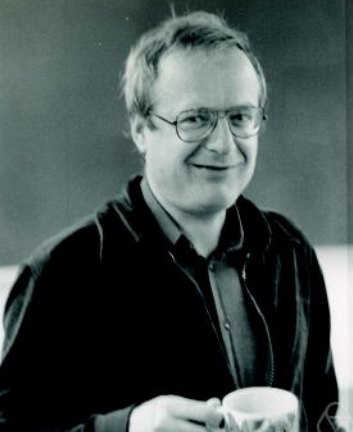
\includegraphics[height=3cm]{Kurzweil-crop}
  \end{center}
    \end{column}
    \begin{column}{0.7\textwidth}
  \begin{itemize}
  \item Fix a finite nonabelian simple group $S$. 
\vskip2mm
\item Suppose the index of $H$ in $G$ is $|G:H| = n$.
\vskip2mm
\item Then the action of $G$ on the cosets of $H$ induces an automorphism of the
group $S^n$ by permutation of coordinates.  
\item
Denote this by  $\phi: G \rightarrow \Aut(S^n)$, 
  and let $\phi(G) = \bar{G} \leq \Aut(S^n)$.  
  \end{itemize}
    \end{column}
\end{columns}
}
\end{frame}

\begin{frame}[label=IEPropsLemma2Alt]{}
%\ifthenelse{\boolean{prezi}}{\FontLarge}{}
\alert{Proof Sketch}
\vskip2mm
  Let $L$ be a group representable lattice such that if $L\cong [H,G]$ and
  $\core_G(H)=1$ then $G$ is a $\cP$-group.  
\vskip4mm
  Since $L$ is representable, $\exists$ a $\cP$-group $G$ with $L
  \cong [H,G]$. 
\vskip4mm
  We apply the idea of Hans Kurzweil twice:
  \begin{itemize}
  \item Fix a finite nonabelian simple group $S$. 
\vskip2mm
\item Suppose the index of $H$ in $G$ is $|G:H| = n$.
\vskip2mm
\item Then the action of $G$ on the cosets of $H$ induces an automorphism of the
group $S^n$ by permutation of coordinates.  
\vskip2mm
\item
Denote this by  $\phi: G \rightarrow \Aut(S^n)$, 
  and let $\phi(G) = \bar{G} \leq \Aut(S^n)$.  
  \end{itemize}
\end{frame}


\begin{frame}[label=IEPropsLemma2Alt]{}
%\ifthenelse{\boolean{prezi}}{\FontLarge}{}
  \begin{itemize}
  \item Fix a finite nonabelian simple group $S$. 
\vskip2mm
\item Suppose the index of $H$ in $G$ is $|G:H| = n$.
\vskip2mm
\item Then the action of $G$ on the cosets of $H$ induces an automorphism of the
group $S^n$ by permutation of coordinates.  
\vskip2mm
\item  The wreath product under this action is the group
  \[
  U := S\wr_\phi G =  S^n \rtimes \bar{G}, % =  S\wr \bar{G},
  \]
  with multiplication
  \[
  (s_1, \dots, s_n, x) (t_1, \dots, t_n, y) = 
  (s_1 t_{x(1)}, \dots, s_nt_{x(n)}, x y),
  \]
  for $s_i, t_i \in S$ and $x, y \in \bar{G}$.
  (From now on, $S^n \rtimes \bar{G} = S^n\bar{G}$.)
\item Denote this by  $\phi: G \rightarrow \Aut(S^n)$, 
  and let $\phi(G) = \bar{G} \leq \Aut(S^n)$.  
  \end{itemize}
\end{frame}


\begin{frame}[fragile,label=IEPropsLemma2Prezi]{}
  \begin{center}
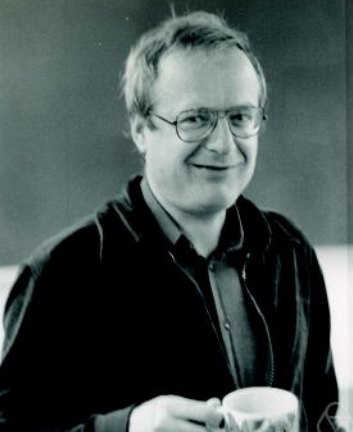
\includegraphics[height=6cm]{Kurzweil-crop}
  \end{center}
\end{frame}


\begin{frame}[label=IEPropsLemma2Wreath]{}
%\ifthenelse{\boolean{prezi}}{\FontLarge}{}
  The wreath product under this action is the group
  \[
  U := S\wr_\phi G =  S^n \rtimes \bar{G}, % =  S\wr \bar{G},
  \]
  with multiplication given by
  \[
  (s_1, \dots, s_n, x) (t_1, \dots, t_n, y) = 
  (s_1 t_{x(1)}, \dots, s_nt_{x(n)}, x y),
  \]
  for $s_i, t_i \in S$ and $x, y \in \bar{G}$.
  (From now on, $S^n \rtimes \bar{G} = S^n\bar{G}$.)
\end{frame}

\begin{frame}[label=IEPropsLemma2]{}
%\ifthenelse{\boolean{prezi}}{\FontLarge}{}
\begin{center}
    {\scalefont{.8}
  \begin{tikzpicture}[scale=.65]
    \node (G) at (3,3) [fill,circle,inner sep=1pt] {}; 
    \draw (G) node [right] {$\bar{G}$};
    \node (H) at (1.75,1.5) [fill,circle,inner sep=1pt] {}; 
    \draw (H) node [left] {$\bar{H}$};
    \node (Sn) at (-5,5) [fill,circle,inner sep=1pt] {}; 
    \draw (Sn) node [left] {$S^n$};
    \node (D) at (-2.5,2.5) [fill,circle,inner sep=1pt] {}; 
    \draw (D) node [right] {$D$};
    \node (DG) at (0.5,5.5) [fill,circle,inner sep=1pt] {}; 
    \draw (DG) node [right] {$D \bar{G}$};
    \node (1) at (0,0) [fill,circle,inner sep=1pt] {}; 
    \draw (1) node [below] {$1$};
    \node (SnG) at (-2,8) [fill,circle,inner sep=1pt] {}; 
    \draw (SnG) node [above] {$U=S^n \bar{G}$};
   \draw
    (G) to [out=190,in=80] (1) to [out=10,in=-100] (G)
    (Sn) to [out=0,in=90] (1) to [out=180,in=-90] (Sn)
    (SnG) to [out=190,in=80] (Sn) to [out=10,in=-100] (SnG)
    (SnG) to [out=0,in=90] (G) to [out=180,in=-90] (SnG);
    \draw[dotted, semithick]
    (G) to [out=190,in=80] (H) to [out=10,in=-100] (G)
    (SnG) to [out=0,in=90] (DG) to [out=180,in=-90] (SnG)
    (Sn) to [out=0,in=90] (D) to [out=180,in=-90] (Sn);
    \draw 
    (-3.75,3.75) node {$\Eq(n)'$}
    (-.75,6.75) node {$L'$}
    (2.3,2.25) node {$L$};
  \end{tikzpicture}
}\end{center}
The interval  $[D, S^n]$ is isomorphic to $\Eq(n)'$, the dual of the lattice of
partitions of an $n$-element set.
\vskip4mm
  The dual lattice $L'$ is an upper interval of $\Sub(U)$, namely,
  $L'\cong [D\bar{G}, U]$. 
\end{frame}

\begin{frame}[label=IEPropsLemma2KeyPoint]{}
%\ifthenelse{\boolean{prezi}}{\FontLarge}{}
  \alert{Key point:} If $H$ is core-free in $G\;$ (equiv., $\ker \phi = 1$), then
\[\text{  $D\bar{G}$ will be core-free in $U$. }\] 
\vskip4mm
Repeating the procedure, with $H_1 :=
  D\bar{G}$ and $L' \cong [H_1, U]$, 
we find $L = L''\cong [D_1 \bar{U}, S^m\bar{U}]$, where $m =
  |U:H_1|$, and $D_1$ is the diagonal subgroup of $S^m$.
  \vskip4mm
  Since $D_1\bar{U}$ is core-free in $S^m \bar{U}$, %(as proved below), 
  it follows by the original hypothesis that $S^m \bar{U} = S \wr
  \bar{U}$ is a $\cP$-group.  
\end{frame}

\begin{frame}[label=IEPropsLemma2]{}
%\ifthenelse{\boolean{prezi}}{\FontLarge}{}
We conclude that a class of groups that does
not include wreath products of the form $S\wr G$, where $S$ is an arbitrary
finite nonabelian simple group, is not a core-free interval enforceable class. 
The class of soluble groups is an example.
\end{frame}




\begin{frame}[fragile,label=Parachutes]{}
%\ifthenelse{\boolean{prezi}}{\FontLarge}{}
\begin{theorem}
The following statements are equivalent:
\begin{enumerate}
\item[(B)] Every finite lattice is isomorphic to
  an interval in the subgroup lattice of a finite group.
\item[(C)]
For every finite lattice $L$ and every finite collection $\sG_1, \dots, \sG_n$
of cf-\IE\ classes of groups,
\[
\exists \; G \in \bigcap\limits_{i=1}^n \sG_i \text{ such that $L \cong [H,G]$
  and $\core_G(H)=1$}.
\]
\item[(D)]
For every finite collection $\sL$ of finite lattices, there exists a finite
group $G$ such that each $L_i \in \sL$ is isomorphic to $[H_i, G]$ for some
core-free subgroup $H_i\leq G$.
\end{enumerate}
\end{theorem}
\end{frame}

\begin{frame}[fragile,label=Parachutes]{}
%\ifthenelse{\boolean{prezi}}{\FontLarge}{}
By (C), the \FLRP\ would have a negative answer if we
could find a collection $\sG_1, \dots, \sG_n$ of cf-\IE\ classes
such that $\bigcap\limits_{i=1}^n \sG_i$ is empty.
\vskip6mm
By (D), it makes sense to consider finite collections of finite lattices and ask
what can be proved about a group $G$ if one assumes that all of these lattices are
isomorphic to upper intervals of $\Sub(G)$. 
\end{frame}

\begin{frame}[fragile,label=Parachutes]{}
%\ifthenelse{\boolean{prezi}}{\FontLarge}{}
\begin{center}
{\scalefont{.8}
\begin{tikzpicture}[scale=0.7]

  \node (G) at (-8,0) [draw,circle,inner sep=1.2pt] {};
  \node (K) at (-11.5,-2) [draw,circle,inner sep=1.2pt] {};
  \node (K1) at (-9.9,-2.8) [draw,circle,inner sep=1.2pt] {};
  \node (K2) at (-8,-3.2) [draw,circle,inner sep=1.2pt] {};
  \node (Kn) at (-5.2,-2.2) [draw,circle,inner sep=1.2pt] {};
  \node (H) at (-8,-7) [draw,circle,inner sep=1.2pt] {};

\draw (-10,-1) node {$L$};
\draw (-9,-1.5) node {$L_1$};
\draw (-8,-1.6) node {$L_2$};
\draw (-6.5,-1) node {$L_n$};
\draw (-6.75,-2.8) node {$\dots$};

%\draw (-8,-8.25) node {(a)};

\draw[semithick] 
   (K) to (H) to (K1)
   (K2) to (H) to (Kn);

\draw [semithick]  
   (G) to [out=-140,in=0] (K)
   (K)  to [out=55,in=185] (G)
   (G) to [out=-105,in=30] (K1)
   (K1) to [out=80,in=-140] (G)
   (G) to [out=-70,in=60] (K2)
   (K2)  to [out=110,in=-110] (G)
   (G) to [out=-10,in=110] (Kn)
   (Kn)  to [out=170,in=-50] (G);
\end{tikzpicture}
}
\end{center}

\end{frame}

\begin{frame}[fragile,label=Parachutes]{}
%\ifthenelse{\boolean{prezi}}{\FontLarge}{}

\begin{center}
{\scalefont{.8}
\begin{tikzpicture}[scale=0.7]
%%% second (labelled) parachute %%%

  \node (Gr) at (1,0) [draw,circle,inner sep=1.2pt] {};
  \node (Kr) at (-2.5,-2) [draw,circle,inner sep=1.2pt] {};
  \node (K1r) at (-0.9,-2.8) [draw,circle,inner sep=1.2pt] {};
  \node (K2r) at (1,-3.2) [draw,circle,inner sep=1.2pt] {};
  \node (Knr) at (3.8,-2.2) [draw,circle,inner sep=1.2pt] {};
  \node (Hr) at (1,-7) [draw,circle,inner sep=1.2pt] {};

\draw (-1,-1) node {$L$};
\draw (0,-1.5) node {$L_1$};
\draw (1,-1.6) node {$L_2$};
\draw (2.5,-1) node {$L_n$};
\draw (2.25,-2.8) node {$\dots$};
%\draw (1,-8.25) node {(b)};


\draw (Gr) node [above] {$G$}
    (Kr) node [left] {$K$}
    (K1r) node [left] {$K_1$}
    (K2r) node [left] {$K_2$}
    (Knr) node [right] {$K_n$}
    (Hr) node [right] {$H$};

\draw[semithick] 
   (Kr) to (Hr) to (K1r)
   (K2r) to (Hr) to (Knr);

\draw [semithick]  
   (Gr) to [out=-140,in=0] (Kr)
   (Kr)  to [out=55,in=185] (Gr)
   (Gr) to [out=-105,in=30] (K1r)
   (K1r) to [out=80,in=-140] (Gr)
   (Gr) to [out=-70,in=60] (K2r)
   (K2r)  to [out=110,in=-110] (Gr)
   (Gr) to [out=-10,in=110] (Knr)
   (Knr)  to [out=170,in=-50] (Gr);
\end{tikzpicture}
}
\end{center}
\end{frame}





\begin{frame}[label=Sevens,shrink=7]{
    Are all lattices with at most 7 elements representable?}
  \note{There are 53 seven element lattices.  We found representations for 43 of
    them without too much trouble.  The last 10 were hard.}
  \begin{columns}
    \begin{column}{0.2\textwidth}
      \begin{center}
        \begin{tikzpicture}[scale=.5]
          % L19
        \node (bottom) at (0,0)  [draw, circle, inner sep=\dotsize] {};
        \node (top) at (0,3)  [draw, circle, inner sep=\dotsize] {};
        \node (11) at (1,1)  [draw, circle, inner sep=\dotsize] {};
        \node (n11) at (-1,1)  [draw, circle, inner sep=\dotsize] {};
        \node (12) at (1,2)  [draw, circle, inner sep=\dotsize] {};
        \node (n12) at (-1,2)  [draw, circle, inner sep=\dotsize] {};
        \node (01) at (0,1)  [draw, circle, inner sep=\dotsize] {};

        \draw[semithick] (bottom) to (11) to (12) to (top) to (n12) to (n11) to (bottom) to (01) to (12);

          \draw (0,-1) node {$L_{19}$};
          \visible<1->{        {\color{red}\draw[font=\large] (.75,-.6) node{$\text{\rlap{$\checkmark$}}$ };}
            \draw (2.5,-.4) node { {\footnotesize Galois}};
            \draw (3.5,-1) node { {\footnotesize correspondence}};
          }
        \end{tikzpicture}
      \end{center}
    \end{column}
    \begin{column}{0.2\textwidth}
      \begin{center}
        \begin{tikzpicture}[scale=.4]
          % L20
      \foreach \j in {0,...,4}
      {
        \node (0\j) at (0,\j)  [draw, circle, inner sep=\dotsize] {};
      }
      \node (152) at (1.5,2)  [draw, circle, inner sep=\dotsize] {};
      \node (n125) at (-1,2.5)  [draw, circle, inner sep=\dotsize] {};
      \draw[semithick] (01) to (02) to (03) to (04) to (n125) to (01) to (00) to (152) to (04);

          \draw (0,-1) node {$L_{20}$};
          \visible<1->{        {\color{red}\draw[font=\large] (1,-.6) node{$\text{\rlap{$\checkmark$}}$ };}
            \draw (3,-.25) node { {\footnotesize Galois}};
            \draw (4.3,-1) node { {\footnotesize correspondence}};
          }
        \end{tikzpicture}
      \end{center}
    \end{column}
  \end{columns}
\vskip-10pt
  \begin{columns}
    \begin{column}{0.2\textwidth}
      \begin{center}
        \begin{tikzpicture}[scale=.4]
          
        \node (bottom) at (0,0)  [draw, circle, inner sep=\dotsize] {};
        \node (top) at (0,5)  [draw, circle, inner sep=\dotsize] {};
        \node (n115) at (-1,1.5)  [draw, circle, inner sep=\dotsize] {};
        \node (015) at (0,1.5)  [draw, circle, inner sep=\dotsize] {};
        \node (115) at (1,1.5)  [draw, circle, inner sep=\dotsize] {};
        \node (n252) at (-2.5,2)  [draw, circle, inner sep=\dotsize] {};
        \node (03) at (0,3)  [draw, circle, inner sep=\dotsize] {};
        \draw[semithick] 
        (bottom) to (n252) to (top)
        (bottom) to (n115) to (03) to (115) to
        (bottom) to (015) to (03) to (top);
       %\draw (-4.5,2.2) node {$L \cong$};



          \draw (0,-1) node {$L_{17}$};
          \visible<1>{        {\color{red}\draw[font=\large] (.75,-.6) node{$\text{\rlap{$\checkmark$}}$ };}
            \draw (3,-.6) node { {\footnotesize filter+ideal}};
          }
          \visible<2->{        {\color{red}\draw[font=\large] (.75,-.6) node{$\text{\rlap{$\checkmark$}}$ };}
            \draw (3,.1) node { {\footnotesize interval in}};
            \draw (3,-.65) node { {\footnotesize $\Sub(G)$}};
          }
        \end{tikzpicture}
      \end{center}
    \end{column}
    \begin{column}{0.2\textwidth}
      \begin{center}
        \begin{tikzpicture}[scale=.5]
          %\newcommand{\dotsize}{1};
\node (0) at (0,0) [draw, circle,inner sep=\dotsize] {};
\node (1) at (-0,1) [draw, circle, inner sep=\dotsize] {};
\node (2) at (1,2) [draw, circle, inner sep=\dotsize] {};
\node (3) at (-1,2) [draw, circle, inner sep=\dotsize] {};
\node (4) at (-0,2) [draw, circle, inner sep=\dotsize] {};
\node (5) at (-0,3) [draw, circle, inner sep=\dotsize] {};
\node (6) at (-0,4) [draw, circle, inner sep=\dotsize] {};
%\draw[font=\scriptsize] (0,-.5) node {[A4, (C2 x C2 x C2 x C2) : A5]};
%\draw[font=\scriptsize] (0,-1) node {SmallGroup(960,11358) Index 80};

\draw[semithick]
(0) to (1)
(0) to (2)
(0) to (3)
(1) to (4)
(2) to (6)
(3) to (6)
(4) to (5)
(5) to (6);

          \draw (0,-.6) node {$L_{13}$};
          \visible<2->{        {\color{red}\draw[font=\large] (.75,-.2) node{$\text{\rlap{$\checkmark$}}$ };}
            \draw (2.5,0) node { {\footnotesize interval in}};
            \draw (2.5,-.6) node { {\footnotesize $\Sub(G)$}};
          }
        \end{tikzpicture}
      \end{center}
    \end{column}

    \begin{column}{0.2\textwidth}
      \begin{center}
        \begin{tikzpicture}[scale=.3]
          % L11 aka L3 
        \node (bottom) at (0,0)  [draw, circle, inner sep=\dotsize] {};
        \node (top) at (2,6)  [draw, circle, inner sep=\dotsize] {};
        \node (n22) at (-2,2)  [draw, circle, inner sep=\dotsize] {};
        \node (22) at (2,2)  [draw, circle, inner sep=\dotsize] {};
        \node (13) at (1,3)  [draw, circle, inner sep=\dotsize] {};
        \node (04) at (0,4)  [draw, circle, inner sep=\dotsize] {};
        \node (44) at (4,4)  [draw, circle, inner sep=\dotsize] {};

        \draw[semithick] (bottom) to (22) to (44) to (top) to (04) to (13) to (22)
        (bottom) to (n22) to (04);
  
          \draw (1,-1) node {$L_{11}$};
          \visible<1->{        {\color{red}\draw[font=\large] (2,-.6) node{$\text{\rlap{$\checkmark$}}$ };}
            \draw (5,-.6) node { {\footnotesize filter+ideal}};
          }
        \end{tikzpicture}
      \end{center}
    \end{column}
  \end{columns}
\vskip-10pt
  \begin{columns}
    \begin{column}{0.2\textwidth}
      \begin{center}
        \begin{tikzpicture}[scale=.5]
          %% ``L9'' is the pentegon with two extra wings.
      \foreach \j in {0,3} 
      { \node (7\j) at (6.5,\j)  [draw, circle, inner sep=\dotsize] {};}
      \node (71) at (7,1.5)  [draw, circle, inner sep=\dotsize] {};
      \node (61) at (6,1.5)  [draw, circle, inner sep=\dotsize] {};
      \node (51) at (5,1.5)  [draw, circle, inner sep=\dotsize] {};
      \foreach \j in {1,2} 
      { \node (8\j) at (7.8,\j)  [draw, circle, inner sep=\dotsize] {};}
      \draw[semithick] (70) to (51) to (73) to (61) to (70) to (71) to (73) to
      (82) to (81) to (70);
      

          \draw (6.5,-1) node {$L_{9}$};
          \visible<1>{        {\color{red}\draw[font=\large] (7,-.6) node{$\text{\rlap{$\checkmark$}}$ };}
            \draw (9,-.4) node { {\footnotesize overalgebra}};
            \draw (9,-1) node { {\footnotesize construction}};
          }
          \visible<2->{        {\color{red}\draw[font=\large] (7,-.6) node{$\text{\rlap{$\checkmark$}}$ };}
            \draw (9,-.4) node { {\footnotesize interval in}};
            \draw (9,-1) node { {\footnotesize $\Sub(G)$}};
          }
        \end{tikzpicture}
      \end{center}
    \end{column}
    \begin{column}{0.2\textwidth}
      \begin{center}
        \begin{tikzpicture}[scale=.5]
          %%  The elusive winged-2x3 %%
      \node (01) at (0,1)  [draw, circle, inner sep=\dotsize] {};
      \foreach \j in {0,2} 
      { \node (1\j) at (1,\j)  [draw, circle, inner sep=\dotsize] {};}

      \foreach \j in {1,3} 
      { \node (2\j) at (2,\j)  [draw, circle, inner sep=\dotsize] {};}
      { \node (32) at (3,2)  [draw, circle, inner sep=\dotsize] {};}
      \draw[semithick] (10) to (01) to (12) to (23) to (32) to (21) to (10) (21) to (12);
      { \node (m11) at (-1,1)  [draw, circle, inner sep=\dotsize] {};}
      \draw[semithick] (10) to (m11) to (23);


          \visible<3>{
            \node (18) at (1.1,1.15)  [draw, circle, red, inner sep=25pt]{};
            \draw[font=\LARGE,color=red] (4.5,1) node {?};
          }
          \draw (1,-.8) node {$L_7$};
                  \end{tikzpicture}
      \end{center}
    \end{column}
  \end{columns}
\end{frame}





\begin{frame}[fragile,label=AOS]{}
%% \vskip2mm
%% \hskip3mm
%% 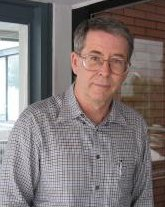
\includegraphics[height=30mm]{Aschbacher3}
%% \begin{center}
%% 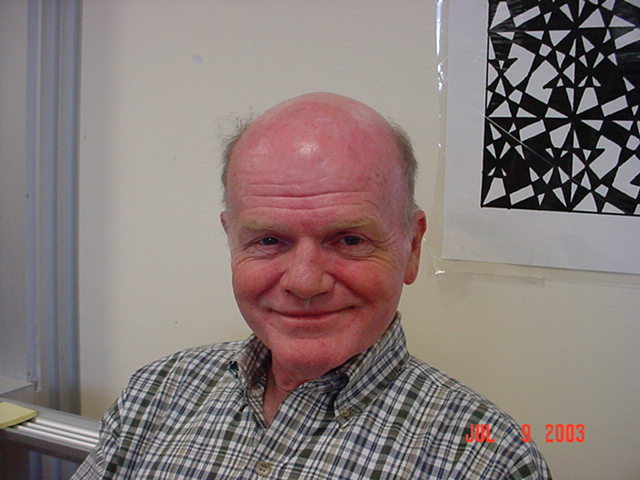
\includegraphics[height=25mm]{ONan}
%% \end{center}
%% \hfill    
%% 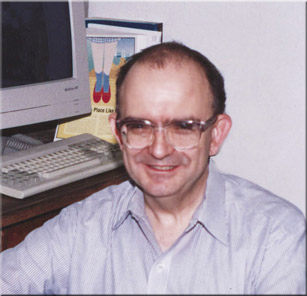
\includegraphics[height=28mm]{Scott}
%% \vskip3mm
\begin{center}
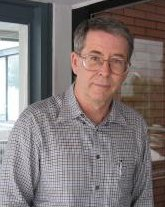
\includegraphics[height=30mm]{Aschbacher3}
\hskip2mm
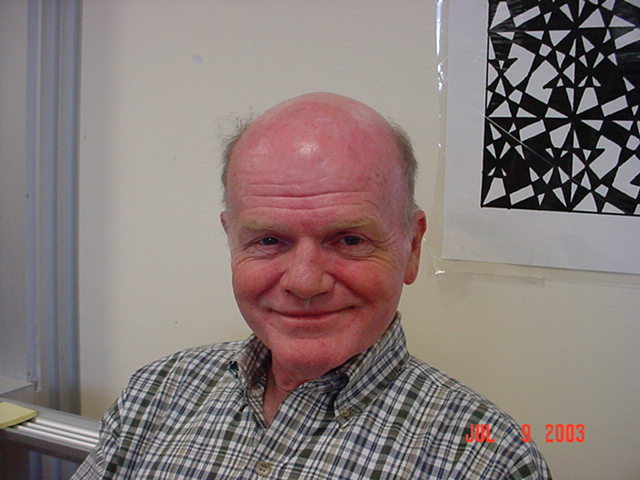
\includegraphics[height=25mm]{ONan}
\hskip2mm
%\hfill    
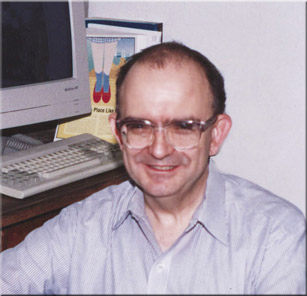
\includegraphics[height=28mm]{Scott}
 \end{center}

\end{frame}



\begin{frame}[fragile,label=Example7elementPreziOld,shrink=5]{The exceptional seven element lattice}
%\ifthenelse{\boolean{prezi}}{\FontLarge}{}
    \begin{theorem}
      \label{thm:except-seven-elem}
      Suppose $H<G$, \hskip2mm $\core_G(H) = 1$, \hskip2mm $L_7 \cong [H,G]$.
      \begin{enumerate}[(i)]
      \item<1-> $G$ is a primitive permutation group.
      \item<1-> If $N\ssubnormal G$, then $C_G(N) = 1$.
      \item<1-> $G$ contains no non-trivial abelian normal subgroup.
      \item<1-> $G$ is not solvable.
      \item<1-> $G$ is subdirectly irreducible.
      \item<1-> With the possible exception of at most one maximal subgroup, %, $M_1$ or $M_2$,
        all proper subgroups in the interval $[H,G]$ are core-free. 
      \end{enumerate}
    \end{theorem}
\end{frame}


\begin{frame}[fragile,label=Example7elementPreziBigFig]{The exceptional seven element lattice}
      \begin{center}
    {\scalefont{1.5}
        \begin{tikzpicture}[scale=1.5]
          %%  The elusive winged-2x3 %%
      \node (01) at (0,1)  [draw, circle, inner sep=\dotsize] {};
      \foreach \j in {0,2} 
      { \node (1\j) at (1,\j)  [draw, circle, inner sep=\dotsize] {};}

      \foreach \j in {1,3} 
      { \node (2\j) at (2,\j)  [draw, circle, inner sep=\dotsize] {};}
      { \node (32) at (3,2)  [draw, circle, inner sep=\dotsize] {};}
      \draw[semithick] (10) to (01) to (12) to (23) to (32) to (21) to (10) (21) to (12);
      { \node (m11) at (-1,1)  [draw, circle, inner sep=\dotsize] {};}
      \draw[semithick] (10) to (m11) to (23);


          \draw (-.25,2.5) node {$L_7$};
        \end{tikzpicture}
}
      \end{center}
\end{frame}

\begin{frame}[label=Example7elementPreziImplications]{}
%\ifthenelse{\boolean{prezi}}{\FontLarge}{}
It is obvious that 
    \begin{itemize}
    \item (ii) $\Rightarrow$ (iii) $\Rightarrow$ (iv), and  
    \item (ii) $\Rightarrow$ (v), but we include these for
      emphasis;
    \item the hard work is in proving (ii) and (vi), but
      the main goal is the pair of restrictions (iii) and (v), which allow us to rule
      out a number of the O'Nan-Scott types describing primitive permutation
      groups. 
  \end{itemize}
\end{frame}



































%%%%%%%%%%%%%%%%%%%%%%%%%%%%%%%%%%%


\begin{frame}[label=conclusion,shrink=5]{Seven element lattices: summary}
  \begin{columns}
    \begin{column}{0.2\textwidth}
      \begin{center}
        \begin{tikzpicture}[scale=.5]

          % L19
        \node (bottom) at (0,0)  [draw, circle, inner sep=\dotsize] {};
        \node (top) at (0,3)  [draw, circle, inner sep=\dotsize] {};
        \node (11) at (1,1)  [draw, circle, inner sep=\dotsize] {};
        \node (n11) at (-1,1)  [draw, circle, inner sep=\dotsize] {};
        \node (12) at (1,2)  [draw, circle, inner sep=\dotsize] {};
        \node (n12) at (-1,2)  [draw, circle, inner sep=\dotsize] {};
        \node (01) at (0,1)  [draw, circle, inner sep=\dotsize] {};

        \draw[semithick] (bottom) to (11) to (12) to (top) to (n12) to (n11) to (bottom) to (01) to (12);

          \draw (0,-1) node {$L_{19}$};
                {\color{red}\draw[font=\large] (1,-.6) node{$\text{\rlap{$\checkmark$}}$ };}
                %\draw[font=\footnotesize] (2.5,-.6) node { Jipsen};

        \end{tikzpicture}
      \end{center}
    \end{column}
    \begin{column}{0.2\textwidth}
      \begin{center}
        \begin{tikzpicture}[scale=.4]
          % L20
      \foreach \j in {0,...,4}
      {
        \node (0\j) at (0,\j)  [draw, circle, inner sep=\dotsize] {};
      }
      \node (152) at (1.5,2)  [draw, circle, inner sep=\dotsize] {};
      \node (n125) at (-1,2.5)  [draw, circle, inner sep=\dotsize] {};
      \draw[semithick] (01) to (02) to (03) to (04) to (n125) to (01) to (00) to (152) to (04);

          \draw (0,-1) node {$L_{20}$};
                {\color{red}\draw[font=\large] (1,-.6) node{$\text{\rlap{$\checkmark$}}$ };}
                %\draw[font=\footnotesize] (3,-.6) node { Jipsen};
        \end{tikzpicture}
      \end{center}
    \end{column}
  \end{columns}

  \begin{columns}
    \begin{column}{0.2\textwidth}
      \begin{center}
        \begin{tikzpicture}[scale=.4]

          
        \node (bottom) at (0,0)  [draw, circle, inner sep=\dotsize] {};
        \node (top) at (0,5)  [draw, circle, inner sep=\dotsize] {};
        \node (n115) at (-1,1.5)  [draw, circle, inner sep=\dotsize] {};
        \node (015) at (0,1.5)  [draw, circle, inner sep=\dotsize] {};
        \node (115) at (1,1.5)  [draw, circle, inner sep=\dotsize] {};
        \node (n252) at (-2.5,2)  [draw, circle, inner sep=\dotsize] {};
        \node (03) at (0,3)  [draw, circle, inner sep=\dotsize] {};
        \draw[semithick] 
        (bottom) to (n252) to (top)
        (bottom) to (n115) to (03) to (115) to
        (bottom) to (015) to (03) to (top);
       %\draw (-4.5,2.2) node {$L \cong$};



          \draw (0,-1) node {$L_{17}$};
                {\color{red}\draw[font=\large] (1,-1) node{$\text{\rlap{$\checkmark$}}$ };}

        \end{tikzpicture}
      \end{center}
    \end{column}

    \begin{column}{0.2\textwidth}
      \begin{center}
        \begin{tikzpicture}[scale=.5]

          %\newcommand{\dotsize}{1};
\node (0) at (0,0) [draw, circle,inner sep=\dotsize] {};
\node (1) at (-0,1) [draw, circle, inner sep=\dotsize] {};
\node (2) at (1,2) [draw, circle, inner sep=\dotsize] {};
\node (3) at (-1,2) [draw, circle, inner sep=\dotsize] {};
\node (4) at (-0,2) [draw, circle, inner sep=\dotsize] {};
\node (5) at (-0,3) [draw, circle, inner sep=\dotsize] {};
\node (6) at (-0,4) [draw, circle, inner sep=\dotsize] {};
%\draw[font=\scriptsize] (0,-.5) node {[A4, (C2 x C2 x C2 x C2) : A5]};
%\draw[font=\scriptsize] (0,-1) node {SmallGroup(960,11358) Index 80};

\draw[semithick]
(0) to (1)
(0) to (2)
(0) to (3)
(1) to (4)
(2) to (6)
(3) to (6)
(4) to (5)
(5) to (6);

          \draw (0,-.6) node {$L_{13}$};
                {\color{red}\draw[font=\large] (1,-.6) node{$\text{\rlap{$\checkmark$}}$ };}

        \end{tikzpicture}
      \end{center}
    \end{column}

    \begin{column}{0.2\textwidth}
      \begin{center}
        \begin{tikzpicture}[scale=.3]

          % L11 aka L3 
        \node (bottom) at (0,0)  [draw, circle, inner sep=\dotsize] {};
        \node (top) at (2,6)  [draw, circle, inner sep=\dotsize] {};
        \node (n22) at (-2,2)  [draw, circle, inner sep=\dotsize] {};
        \node (22) at (2,2)  [draw, circle, inner sep=\dotsize] {};
        \node (13) at (1,3)  [draw, circle, inner sep=\dotsize] {};
        \node (04) at (0,4)  [draw, circle, inner sep=\dotsize] {};
        \node (44) at (4,4)  [draw, circle, inner sep=\dotsize] {};

        \draw[semithick] (bottom) to (22) to (44) to (top) to (04) to (13) to (22)
        (bottom) to (n22) to (04);
  \draw (1,-1) node {$L_{11}$};
                {\color{red}\draw[font=\large] (2.3,-1) node { $\text{\rlap{$\checkmark$}}$};}

        \end{tikzpicture}
      \end{center}
    \end{column}

  \end{columns}


  \begin{columns}

    \begin{column}{0.2\textwidth}
      \begin{center}
        \begin{tikzpicture}[scale=.5]

          %% ``L9'' is the pentegon with two extra wings.
      \foreach \j in {0,3} 
      { \node (7\j) at (6.5,\j)  [draw, circle, inner sep=\dotsize] {};}
      \node (71) at (7,1.5)  [draw, circle, inner sep=\dotsize] {};
      \node (61) at (6,1.5)  [draw, circle, inner sep=\dotsize] {};
      \node (51) at (5,1.5)  [draw, circle, inner sep=\dotsize] {};
      \foreach \j in {1,2} 
      { \node (8\j) at (7.8,\j)  [draw, circle, inner sep=\dotsize] {};}
      \draw[semithick] (70) to (51) to (73) to (61) to (70) to (71) to (73) to
      (82) to (81) to (70);
      

          \draw (6.5,-1) node {$L_{9}$};
            {\color{red}\draw[font=\large] (7.5,-.6) node{$\text{\rlap{$\checkmark$}}$ };}
            %\draw[font=\large] (9.3,-.6) node { {\footnotesize Freese}};
        \end{tikzpicture}
      \end{center}
    \end{column}


    \begin{column}{0.2\textwidth}
      \begin{center}
        \begin{tikzpicture}[scale=.5]

          %%  The elusive winged-2x3 %%
      \node (01) at (0,1)  [draw, circle, inner sep=\dotsize] {};
      \foreach \j in {0,2} 
      { \node (1\j) at (1,\j)  [draw, circle, inner sep=\dotsize] {};}

      \foreach \j in {1,3} 
      { \node (2\j) at (2,\j)  [draw, circle, inner sep=\dotsize] {};}
      { \node (32) at (3,2)  [draw, circle, inner sep=\dotsize] {};}
      \draw[semithick] (10) to (01) to (12) to (23) to (32) to (21) to (10) (21) to (12);
      { \node (m11) at (-1,1)  [draw, circle, inner sep=\dotsize] {};}
      \draw[semithick] (10) to (m11) to (23);



          \visible<2>{\node (18) at (1,1.3)  [draw, circle, red, inner sep=25pt] {};}

          \draw (1,-.8) node {$L_7$};
        \end{tikzpicture}
      \end{center}
    \end{column}
  \end{columns}
\end{frame}


\frame[label=MO,shrink=5]{
  \frametitle{Has anyone seen this lattice?}
  \begin{center}
    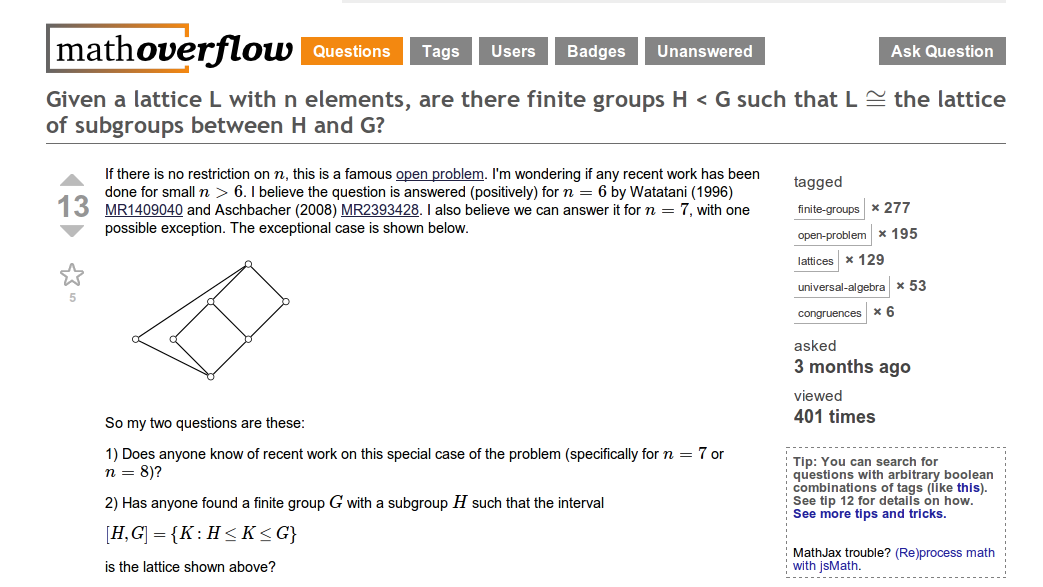
\includegraphics[height=2.8in]{MOquestion201204}
  \end{center}
}  



\begin{frame}[fragile,label=NewConclusion,shrink=5]{The exceptional seven element lattice}
%  \frametitle{Interval enforceable properties}
      \begin{center}
        \begin{tikzpicture}[scale=.5]
          %%  The elusive winged-2x3 %%
      \node (01) at (0,1)  [draw, circle, inner sep=\dotsize] {};
      \foreach \j in {0,2} 
      { \node (1\j) at (1,\j)  [draw, circle, inner sep=\dotsize] {};}

      \foreach \j in {1,3} 
      { \node (2\j) at (2,\j)  [draw, circle, inner sep=\dotsize] {};}
      { \node (32) at (3,2)  [draw, circle, inner sep=\dotsize] {};}
      \draw[semithick] (10) to (01) to (12) to (23) to (32) to (21) to (10) (21) to (12);
      { \node (m11) at (-1,1)  [draw, circle, inner sep=\dotsize] {};}
      \draw[semithick] (10) to (m11) to (23);


          \draw (1,-.8) node {$L_7$};
        \end{tikzpicture}
      \end{center}
    \begin{theorem}
      \label{thm:except-seven-elem}
      Suppose $H<G$, \hskip2mm $\core_G(H) = 1$, \hskip2mm $L_7 \cong [H,G]$.
      \begin{enumerate}[(i)]
      \item<1-> $G$ is a primitive permutation group.
      \item<1-> If $N\ssubnormal G$, then $C_G(N) = 1$.
      \item<1-> $G$ contains no non-trivial abelian normal subgroup.
      \item<1-> $G$ is not solvable.
      \item<1-> $G$ is subdirectly irreducible.
      \item<1-> With the possible exception of at most one maximal subgroup, %, $M_1$ or $M_2$,
        all proper subgroups in the interval $[H,G]$ are core-free. 
      \end{enumerate}
    \end{theorem}

  \note{  It is obvious that 
    \begin{itemize}
    \item (ii) $\Rightarrow$ (iii) $\Rightarrow$ (iv), and  
    \item (ii) $\Rightarrow$ (v), but we include these for
      emphasis;
    \item the hard work is in proving (ii) and (vi), but
      the main goal is the pair of restrictions (iii) and (v), which allow us to rule
      out a number of the O'Nan-Scott types describing primitive permutation
      groups. 
  \end{itemize}}
\end{frame}

%%% NEW STUFF %%%


\begin{frame}[fragile,label=SubgroupLatticeBasics]{Subgroup Lattice Basics}
Let $U$ and $H$ be subgroups of a finite group.
  \begin{itemize}
  \item<1-> By $UH$ we mean the \emph{set} $\{ u h \mid u\in U, h\in H\}$.\\[6pt]
  \item<2-> $U \join V = \<U,H\>$ means the group generated by $U$ and $H$.\\[6pt]
  \item<3-> $UH \subseteq \<U,H\>$ and 
    equality holds iff $U$ and $H$ permute: 
    \[
    UH = \<U,H\> \quad \Leftrightarrow \quad U H = H U.
    \]
  \end{itemize}
\visible<4->{
\begin{center}
  \begin{tikzpicture}[scale=.4]
    \node (H) at (4,4) [fill,circle,inner sep=\dotsize] {}; \draw (H) node [right] {$H$};
    \node (U) at (-4,4) [fill,circle,inner sep=\dotsize] {}; \draw (U) node [left] {$U$};
    \node (U0) at (0,0) [fill,circle,inner sep=\dotsize] {}; 
    \draw (1.5,-.75) node {$U_0 = U\cap H$};
    \node (UH) at (0,8) [fill,circle,inner sep=\dotsize] {}; \draw (UH) node [above] {$\<U,H\>$};
 \draw
    (U) to [out=-10,in=100] (U0) to [out=170,in=-80] (U)
    (UH) to [out=-10,in=100] (H) to [out=170,in=-80] (UH)
    (H) to [out=190,in=80] (U0) to [out=10,in=-100] (H)
    (UH) to [out=190,in=80] (U) to [out=10,in=-100] (UH);
    \visible<5->{\shade[top color=olivegreen,bottom color=gray!50] 
      (U) to [out=-10,in=100] (U0) to [out=170,in=-80] (U);
      \draw (-7,0) node {$[U_0,U]:=\{V \mid U_0 \leq V \leq U\}$};}
    % \visible<6->{  \shade[top color=blue,bottom color=gray!50] 
    %   (UH) to [out=-10,in=100] (H) to [out=170,in=-80] (UH);
    %   \draw (7,6) node {$[H, \<U,H\>]$};}
    \visible<5->{ \node (V) at (-1.6,1.8) [fill,circle,inner sep=\dotsize] {};
      \draw (-2,2) node {$V$};}
    \end{tikzpicture}
\end{center}
}
\end{frame}


\begin{frame}[fragile,label=IntervalIsomorphisms,shrink=5]{Interval Isomorphisms}
  \begin{columns}
    \begin{column}{0.3\textwidth}
      \begin{center}
        \begin{tikzpicture}[scale=.3]
              \node (H) at (4,4) [draw,circle,inner sep=\dotsize] {}; \draw (H) node [right] {$H$};
    \node (U) at (-4,4) [draw,circle,inner sep=\dotsize] {}; \draw (U) node [left] {$U$};
    \node (U0) at (0,0) [draw,circle,inner sep=\dotsize] {}; 
    \draw (1.5,-.75) node {$U_0 = U\cap H$};
    \node (UH) at (0,8) [draw,circle,inner sep=\dotsize] {}; \draw (UH) node
    [above] {$UH$};
 \draw
    (U) to [out=-10,in=100] (U0) to [out=170,in=-80] (U)
    (UH) to [out=-10,in=100] (H) to [out=170,in=-80] (UH)
    (H) to [out=190,in=80] (U0) to [out=10,in=-100] (H)
    (UH) to [out=190,in=80] (U) to [out=10,in=-100] (UH);

    \visible<1>{\shade[top color=olivegreen,bottom color=gray!-45] 
      (U) to [out=-10,in=100] (U0) to [out=170,in=-80] (U);}
    \visible<4->{
      \fill[color=olivegreen] 
      (U) to [out=-10,in=100] (U0) to [out=170,in=-80] (U);}
    \visible<1,4->{  \shade[top color=olivegreen,bottom color=gray!-45] 
      (UH) to [out=-10,in=100] (H) to [out=170,in=-80] (UH);}
    \visible<5->{\fill[color=orange]    
      (H) to [out=190,in=80] (U0) to [out=10,in=-100] (H);}
    \visible<5->{\shade[top color=orange,bottom color=gray!0]    
      (UH) to [out=190,in=80] (U) to [out=10,in=-100] (UH);}
       \end{tikzpicture}
      \end{center}
    \end{column}
    \begin{column}{0.8\textwidth}
      \begin{itemize}
      \item<1-> If $H\subnormal \<U, H\>$, then %\\[4pt]
        $UH = \<U, H\> \; \text{ and } \; [U_0, U] \cong [H, UH]$.\vskip2mm
        \item<2-> Instead of $H\subnormal \<U,H\>$, assume only
          $UH = \<U,H\>$ and define   
          \begin{equation*}
            %      \label{eq:dedekind-1}
            [U_0, U]^H := \{ V\in [U_0,U] \mid VH = HV\},
          \end{equation*}
          the \alert{$H$-permuting subgroups}.
          \vskip2mm 
        \item<3-> If $U \subnormal UH$,
          define
          \begin{equation*}
            %  \label{eq:dedekind-2}
            [U_0, U]_H := \{ V\in [U_0,U] \mid H\leq N_{UH}(V)\}, 
          \end{equation*}
          the \alert{$H$-invariant subgroups}: 
          $V^h = V \; (\forall h\in H)$.
      \end{itemize}
    \end{column}
  \end{columns}

\vskip4mm

  \visible<4->{
    \begin{lemma}
      \label{lemma-wjd-4}
      \begin{enumerate}
      \item $[H, UH]  \cong  [U_0, U]^H \leq [U_0, U]$ 
       % \only<6>{ and \hskip2mm $[U, UH] \cong  [U_0, H]^U \leq [U_0, H]$.}
\\[6pt]
      \item If $U \subnormal UH$, then  $[U_0, U]_H  = [U_0, U]^H \leq [U_0, U]$.\\[6pt]
      \item If $H \subnormal UH$,  then  $[U_0, U]_H  = [U_0, U]^H = [U_0, U]$.
      \end{enumerate}
    \end{lemma}
}
\note{
  \begin{itemize}
  \item 
  Since $G=UH$ is a group, the hypothesis of (ii) is equivalent to
$H\leq N_G(U)$, and the hypothesis of (iii) is equivalent to $U\leq N_G(H)$.
\item Part (i) of the lemma says that when two subgroups permute, we can
identify the interval above either one of them with the sublattice of
subgroups below the other that permute with the first.
\item Part (ii) is similar except we identify the interval above $H$ with
the  sublattice of $H$-invariant subgroups below $U$.
\item Once we have proved (i), the
proof of (iii) follows trivially from the Noether isomorphism theorem.
  \end{itemize}}

\end{frame}


%%%%%% Example %%%%%%%%%
\begin{frame}[fragile,label=ExampleOfPermutingIso,shrink=5]{Example 1}

  \begin{itemize}
  \item<1-> Consider $G\cong C_3 \times S_3$, say,
    \[G = \<a,b,c \mid a^2, b^3, c^3, [b,a], [c,b], c^{-1}a^{-1}a^c\>\]
\item<2->The subgroups 
\[U = \<a,b\> \cong C_6, \qquad H = \<bc\>\cong C_3\]
permute ($UH = HU$) but neither one normalizes the other.
  \end{itemize}
\vskip4mm
\visible<2->{
\begin{center}
  {\scalefont{.8}
    \begin{tikzpicture}[scale=.4]
      
        \node (U0) at (0,0)  [draw, circle, inner sep=\dotsize] {};
        \draw (U0) node [below] {$U_0 = 1$};
        \node (UH) at (0,8)  [draw, circle, inner sep=\dotsize] {};
        \draw (UH) node [above] {$UH = \<a,b,c\>$};
        \node (V) at (-2.5,2)  [draw, circle, inner sep=\dotsize] {};
        \node (W) at (-.5,3)  [draw, circle, inner sep=\dotsize] {};
        \node (U) at (-3,5)  [draw, circle, inner sep=\dotsize] {};
        \draw (U) node [left] {$U=\<a,b\>$};
        \node (H) at (2.5,3)  [draw, circle, inner sep=\dotsize] {};
        \draw (H) node [right] {$H=\<bc\>$};
        \node (K) at (2,6)  [draw, circle, inner sep=\dotsize] {};

        \draw[semithick] 
        (U0) to (V) to (U) to (W) to (U0) to (H) to (K) to (UH) to (U);
       %\draw (-4.5,2.2) node {$L \cong$};



        \visible<3->{
          \draw (V) node [left] {$\<a\>$};
          \draw (W) node [right] {$\<b\>$};
          \draw (K) node [right] {$\<b,c\>\cong C_3 \times C_3$};
        }
        \visible<4->{\draw[semithick,dotted] (K) to (W);}
    \end{tikzpicture}
  }
\end{center}
}
  \begin{itemize}
  \item<4-> Three of the four subgroups of $U$ permute with $H$.
\\[4pt] As the lemma predicts, $U\cap \<b, c\> = \<b\>$.
  \end{itemize}
\end{frame}


%%%%%% Example2 %%%%%%%%%
\begin{frame}[fragile,label=ExampleOfPermutingIso,shrink=5]{Example 2}

  \begin{itemize}
  \item<1-> The group $S_4$ has subgroups $U\cong D_8$ and $H\cong C_3$ which 
    permute but neither one normalizes the other.
  \end{itemize}
\vskip4mm
\visible<2->{
\begin{center}
  {\scalefont{.8}
    \begin{tikzpicture}[scale=.4]
      
        \node (U0) at (0,0)  [draw, circle, inner sep=\dotsize] {};
        \draw (U0) node [below] {$H_0 = 1$};
        \node (UH) at (3,13)  [draw, circle, inner sep=\dotsize] {};
        \draw (UH) node [above] {$HK = S_4$};
        \node (V) at (-3,5)  [draw, circle, inner sep=\dotsize] {};
        \node (W) at (1,5)  [draw, circle, inner sep=\dotsize] {};
        \node (U) at (-2,8)  [draw, circle, inner sep=\dotsize] {};
        \draw (U) node [left] {$H\cong D_8$};
        \node (H) at (5,5)  [draw, circle, inner sep=\dotsize] {};
        \draw (H) node [right] {$K \cong C_3$};
        \node (A4) at (2,10)  [draw, circle, inner sep=\dotsize] {};
        \draw (A4) node [right] {$A_4$};
        \node (S3) at (6,10)  [draw, circle, inner sep=\dotsize] {};
        \draw (S3) node [right] {$S_3$};
        \node (a) at (-3.6,3)  [draw, circle, inner sep=\dotsize] {};
        \node (b) at (-2,3)  [draw, circle, inner sep=\dotsize] {};
        \node (c) at (-1,4)  [draw, circle, inner sep=\dotsize] {};
        \node (d) at (-0,4)  [draw, circle, inner sep=\dotsize] {};
        \node (e) at (-1.5,6)  [draw, circle, inner sep=\dotsize] {};
        \node (f) at (0,6)  [draw, circle, inner sep=\dotsize] {};

        \draw[semithick] 
        (U0) to (a) to (V) to (b) to (U0) to (c) to (V) to (U) to (e) to (c) to
        (f) to (d) to (U0) to (W) to (f) to (U) (UH) to (A4) to (H) to (S3)
        to (UH);
        \draw[semithick,dotted] 
        (U) to (UH)   (U0) to (H);
       %\draw (-4.5,2.2) node {$L \cong$};



      \visible<3->{\draw[semithick,dotted]
        (V) to (A4) (W) to (S3);
        \draw (V) node [left] {$V\cong C_2\times C_2$};
        \draw (W) node [right] {$W\cong C_2 $};
      }
    \end{tikzpicture}
  }
\end{center}
}
\begin{itemize}
\item<2-> Only four subgroups of $U$ permute with $H$%
\visible<3->{, including
    \[ 
U\cap A_4 \cong C_2\times C_2, \qquad U \cap S_3 \cong C_2.
    \]
  }
\end{itemize}
\end{frame}


\begin{frame}[fragile,label=Dedekind]{}
%\vskip-1cm
%The proof relies on Dedekind's modular law for subgroups.
\vskip3mm
\begin{theorem}[Dedekind's Rule]
  \label{lemma-dedekind}
Let $A, B, C$ be subgroups of $G$ with $A\leq B$.  Then,
\[
A(C\cap B) = AC \cap B \quad \text{ and }
\quad (C\cap B)A = CA \cap B.
\]
\end{theorem}
\vskip3mm
In other words, no pentagons.
\vskip3mm
\hfill    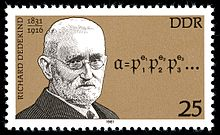
\includegraphics[height=25mm]{Dedekind-stamp}
\note{Draw picture of $N_5$ with $A\leq B$ to demonstrate that it contradicts Dedekind's rule.}
\end{frame}


\begin{frame}[fragile,label=ProofOfIntervalIsomorphism,shrink=5]{Proof of Interval Isomorphism Lemma}
  \begin{columns}
    \begin{column}{0.45\textwidth}
      \begin{claim}[1]
      $[H, UH]  \cong  [U_0, U]^H$ via
        \begin{align*}
          \phi: \;& [H, UH] \ni X \mapsto U\cap X \in [U_0, U]^H\\[6pt]
          \psi: \;& [U_0, U]^H \ni V \mapsto VH \in [H, UH].
        \end{align*}
      \end{claim}
    \end{column}
    \begin{column}{0.55\textwidth}
      \begin{center}
        {\scalefont{.75}
          \begin{tikzpicture}[scale=.35]
                \node (H) at (4,4) [draw,circle,inner sep=\dotsize] {}; \draw (H) node [right] {$H$};
    \node (U) at (-4,4) [draw,circle,inner sep=\dotsize] {}; \draw (U) node [left] {$U$};
    \node (U0) at (0,0) [draw,circle,inner sep=\dotsize] {}; 
    \draw (1.5,-.75) node {$U_0 = U\cap H$};
    \node (UH) at (0,8) [draw,circle,inner sep=\dotsize] {}; \draw (UH) node
    [above] {$UH$};
 \draw
    (U) to [out=-10,in=100] (U0) to [out=170,in=-80] (U)
    (UH) to [out=-10,in=100] (H) to [out=170,in=-80] (UH)
    (H) to [out=190,in=80] (U0) to [out=10,in=-100] (H)
    (UH) to [out=190,in=80] (U) to [out=10,in=-100] (UH);

            \fill[color=olivegreen] 
            (U) to [out=-10,in=100] (U0) to [out=170,in=-80] (U);
            \shade[top color=olivegreen,bottom color=gray!-45] 
            (UH) to [out=-10,in=100] (H) to [out=170,in=-80] (UH);
            \node (V) at (-2.3,2.5) [fill,circle,inner sep=\dotsize] {}; \draw (V) node [left] {$V$};
            \node (VH) at (1.7,6.5){};
            \node (X) at (2.5,5.3) [fill,circle,inner sep=\dotsize] {}; \draw (X) node [right] {$X$};
            \node (UcapX) at (-1.5,1.3){};
            \draw[semithick,dotted] 
            (V) to [out=65,in=-155] (VH)
            (X) to [out=-155,in=65] (UcapX);
          \end{tikzpicture}
        }
      \end{center}
    \end{column}
  \end{columns}
\vskip5mm
  %% \begin{columns}
  %%   \begin{column}{0.6\textwidth}
      \begin{proof}
        \begin{itemize}
        \item[1.] For $X\in [H, UH]$,
          check $U\cap X \in [U_0, U]^H$ by Dedekind's rule.\vskip6pt
        \item[2.] For $V\in [U_0, U]^H$, $VH$ is a group in $[H, UH]$.\vskip6pt
        \item[3.]  Check $\psi \phi$ and $\phi \psi$ are the identity maps. \vskip6pt
        \item[4.] Check $\phi$ and $\psi$ are order preserving.
        \end{itemize}
      \end{proof}

\end{frame}
%% \begin{frame}[fragile,label=ProofOfIntervalIsomorphism,shrink=5]{Proof of Interval Isomorphism Lemma}
%%         \begin{computations}
%%       \begin{itemize}
%%       \item[1.] $(U\cap X) H = UH \cap X= HU \cap X = H(U \cap X)$\vskip10pt
%%       \item[3.] $\psi \phi (X) = (U\cap X)H =UH \cap X = X.$\\[4pt]
%%         $\phi \psi(V)= VH \cap U =V(H\cap U)= V$.\vskip10pt
%%       \item[4.] $X\leq Y \; \Rightarrow \; U\cap X \leq U\cap Y$\\[4pt]
%%         $V\leq W \; \Rightarrow \; VH \leq WH$.
%%       \end{itemize}
%%         \end{computations}
%% \end{frame}

%%% Prezi version %%%
\begin{frame}[fragile,label=ComputationsForProofOfIntervalIsomorphism,shrink=5]{}
 $(U\cap X) H = UH \cap X= HU \cap X = H(U \cap X)$
\end{frame}
\begin{frame}[fragile,label=ComputationsForProofOfIntervalIsomorphism,shrink=5]{}
  $\psi \phi (X) = (U\cap X)H =UH \cap X = X$\\[4pt]
  $\phi \psi(V)= VH \cap U =V(H\cap U)= V$
\end{frame}
\begin{frame}[fragile,label=ComputationsForProofOfIntervalIsomorphism,shrink=5]{}
$X\leq Y \; \Rightarrow \; U\cap X \leq U\cap Y$\\[4pt]
  $V\leq W \; \Rightarrow \; VH \leq WH$.
\end{frame}


      %% \item<1-> 

      %% {\bf Claim 1:} $[H, UH]  \cong  [U_0, U]^H \leq [U_0, U]$.

\begin{frame}[fragile,label=ProofOfIntervalIsomorphism,shrink=5]{Proof of Interval Isomorphism Lemma}
  \begin{columns}
    \begin{column}{0.45\textwidth}
      \begin{claim}[2]
      $[U_0, U]^H$ is a sublattice of $[U_0,U]$.
      \end{claim}
    \end{column}
    \begin{column}{0.55\textwidth}
       \begin{center}
        {\scalefont{.8}
          \begin{tikzpicture}[scale=.35]
                \node (H) at (4,4) [draw,circle,inner sep=\dotsize] {}; \draw (H) node [right] {$H$};
    \node (U) at (-4,4) [draw,circle,inner sep=\dotsize] {}; \draw (U) node [left] {$U$};
    \node (U0) at (0,0) [draw,circle,inner sep=\dotsize] {}; 
    \draw (1.5,-.75) node {$U_0 = U\cap H$};
    \node (UH) at (0,8) [draw,circle,inner sep=\dotsize] {}; \draw (UH) node
    [above] {$UH$};
 \draw
    (U) to [out=-10,in=100] (U0) to [out=170,in=-80] (U)
    (UH) to [out=-10,in=100] (H) to [out=170,in=-80] (UH)
    (H) to [out=190,in=80] (U0) to [out=10,in=-100] (H)
    (UH) to [out=190,in=80] (U) to [out=10,in=-100] (UH);

            \fill[color=olivegreen] 
            (U) to [out=-10,in=100] (U0) to [out=170,in=-80] (U);
            \shade[top color=olivegreen,bottom color=gray!-45] 
            (UH) to [out=-10,in=100] (H) to [out=170,in=-80] (UH);
            \node (V) at (-2.3,1.7) [fill,circle,inner sep=\dotsize] {};
            \draw (V) node [left] {$V$};
            \node (W) at (-1.5,2)[fill,circle,inner sep=\dotsize] {};
            \draw (W) node [right] {$W$};
          \end{tikzpicture}
        }
      \end{center}
 %     \vskip1cm
    \end{column}
  \end{columns}
       \begin{proof}
          Fix $V, W \in [U_0, U]^H$.\vskip6pt
          \begin{itemize}
          \item[1.] Check $V \join W = \<V, W\>$ permutes with $H$. (easy)\vskip10pt
          \item[2.]Check $V \cap W$ permutes with $H$.
          \end{itemize}
          \end{proof}
%% To prove (ii), assuming $U\subnormal G$, we show that if $U_0 \leq V \leq U$,
%% then $VH = HV$ if and only if $H\leq N_G(V)$.
%% If $H\leq N_G(V)$, then $VH = HV$ (even when $U \notsubnormal G$).
%% Suppose $VH = HV$.  We must show $(\forall v\in V)\, (\forall h\in H)\; hvh^{-1}\in
%% V$.  Fix $v\in V, \, h\in H$.  Then, $hv = v'h'$ for some $v'\in V,\, h'\in H$, since
%% $VH = HV$.  Therefore, $v' h' h^{-1} = hvh^{-1} = u$ for some $u\in U$, since
%% $H\leq N_G(U)$. This proves that $hvh^{-1}\in VH\cap U = V(H\cap U) = VU_0 = V$, as
%% desired.
 
\end{frame}

%% \begin{frame}[fragile,label=ProofOfIntervalIsomorphism,shrink=5]{Proof of Interval Isomorphism Lemma}
%%         \begin{computations}
%%       \begin{itemize}
%%       \item[2.] Fix $x \in V \cap W$ and $h\in H$.\\[6pt]  
%%           {\bf To Show:} $xh = h'x'$ for some $h'\in H, \, x'\in V\cap W$.\\[6pt]
%%           Since $V$ and $W$ permute with $H$, 
%%           \[xh = h_1 v \quad \text{ and } \quad xh = h_2 w\]
%%           for some $h_i\in H,\,v \in V,\, w \in W$.\\[10pt]
%%           {\bf Exercise:} Check that this puts $v\in V \cap HW \leq V \cap W$. 
%%           \note{
%%             \[h_1 v = h_2 w \;\Rightarrow \; v = h_1^{-1}h_2 w \in HW.\]
%%             So $v\in V \cap HW$, which is below $V$ and
%%             $U\cap HW = \phi \psi(W) = W$.  
%%             \[\therefore \quad v \in V \cap HW \leq V \cap W.\]
%%             which proves $xh = h_1 v$ for $h_1\in H$ and $v \in V\cap W$, as
%%             desired.}
%%       \end{itemize}
%%         \end{computations}
%% \end{frame}

%%% Prezi version %%%
\begin{frame}[fragile,label=ComputationsForProofOfIntervalIsomorphism,shrink=5]{}
      Fix $x \in V \cap W$ and $h\in H$.\\[6pt]  
      {\bf To Show:} $xh = h'x'$ for some $h'\in H, \, x'\in V\cap W$.
\end{frame}
\begin{frame}[fragile,label=ComputationsForProofOfIntervalIsomorphism,shrink=5]{}
          Since $V$ and $W$ permute with $H$, 
          \[xh = h_1 v \quad \text{ and } \quad xh = h_2 w\]
          for some $h_i\in H,\,v \in V,\, w \in W$.
\end{frame}
\begin{frame}[fragile,label=ComputationsForProofOfIntervalIsomorphism,shrink=5]{}
          {\bf Exercise:} Check that this puts $v\in V \cap HW \leq V \cap W$. 
\end{frame}
\begin{frame}[fragile,label=ComputationsForProofOfIntervalIsomorphism,shrink=5]{}
            \[h_1 v = h_2 w \;\Rightarrow \; v = h_1^{-1}h_2 w \in HW.\]
            So $v\in V \cap HW$, which is below $V$ and
            $U\cap HW = \phi \psi(W) = W$.  
            \[\therefore \quad v \in V \cap HW \leq V \cap W.\]
            which proves $xh = h_1 v$ for $h_1\in H$ and $v \in V\cap W$, as
            desired.
\end{frame}


\begin{frame}[fragile,label=L7second,shrink=5]{}
  \begin{center}
    {\scalefont{.75}
      \begin{tikzpicture}[scale=.7]
              \node (J1) at (0,1)  [draw, circle, inner sep=\dotsize] {};
      \draw (.36, 1) node {$J_1$};
      \node (H) at (1,0)  [draw, circle, inner sep=\dotsize] {};
      \draw (1.16, -.2) node {$H$};
      \node (M2) at (1,2)  [draw, circle, inner sep=\dotsize] {};
      \draw (1.4, 2) node {$M_2$};
      \node (J2) at (2,1)  [draw, circle, inner sep=\dotsize] {};
      \draw (2.2, .8) node {$J_2$};
      \node (G) at (2,3)  [draw, circle, inner sep=\dotsize] {};
      \draw (2.3, 3.1) node {$G$};
      \node (M1) at (3,2)  [draw, circle, inner sep=\dotsize] {};
      \draw (3.35, 2) node {$M_1$};
      \node (K) at (-1,1.2)  [draw, circle, inner sep=\dotsize] {};
      \draw (-1.28, 1.15) node {$K$};

      \draw[semithick] (H) to (J1) to (M2) to (G) to (M1) to (J2) to (H) (J2) to (M2);
      \draw[semithick] (H) to (K) to (G);

      \end{tikzpicture}
    }
  \end{center}

\begin{theorem}
\label{thm:except-seven-elem}
Suppose $H<G$, $\core_G(H) = 1$, and 
$L_7 \cong [H,G]$.  Then
\begin{enumerate}[(i)]
\item<1-> $G$ is a primitive permutation group.
\item<1-> If $N\ssubnormal G$, then $C_G(N) = 1$.
\item<1-> $G$ contains no non-trivial abelian normal subgroup.
\item<1-> $G$ is not solvable.
\item<1-> $G$ is subdirectly irreducible.
\item<1-> With the possible exception of at most one maximal subgroup, $M_1$ or $M_2$,
  all proper subgroups in the interval $[H,G]$ are core-free. 

%% The three subgroups in $[H,G]$ which cover $H$ (the atoms) are
%%   core-free.  At least one two of the three maximal subgroups (the co-atoms) in
%%   the interval are core-free. 
\end{enumerate}
\end{theorem}
%% \note{  It is obvious that 
%%   \begin{itemize}
%%   \item (ii) $\Rightarrow$ (iii) $\Rightarrow$ (iv), and  
%% \item (ii) $\Rightarrow$ (v), but we include these for
%%   emphasis;
%% \item the hard work is in proving (ii) and (vi), but
%%   the main goal is the pair of restrictions (iii) and (v), which allow us to rule
%%   out a number of the O'Nan-Scott types describing primitive permutation
%%   groups. 
%%   \end{itemize}}
\end{frame}

\begin{frame}[fragile,label=IdeaOfL7Proof,shrink=5]{Example Application}
    %% \begin{column}{0.3\textwidth}
      \begin{center}
        {\scalefont{.78}
          \begin{tikzpicture}[scale=1]
      \node (N) at (-.6,0)  [draw, circle, inner sep=1pt] {};
      \draw (-.9, 0) node {$N$};
      \node (NcapH) at (.2,-1)  [draw, circle, inner sep=1pt] {};
      \node (J1) at (0.2,1)  [draw, circle, inner sep=1pt] {};
      \draw (-.15, 1.05) node {$J_1$};
      \node (H) at (1,0)  [draw, circle, inner sep=1pt] {};
      \draw (1.16, -.2) node {$H$};
      \node (M2) at (1,2)  [draw, circle, inner sep=1pt] {};
      \draw (.6, 2.1) node {$M_2$};
      \node (J2) at (1.8,1)  [draw, circle, inner sep=1pt] {};
      \draw (1.35, 1.) node {$J_2$};
      \node (G) at (1.8,3)  [draw, circle, inner sep=1pt] {};
      \draw (2.1, 3.1) node {$G$};
      \node (M1) at (2.6,2)  [draw, circle, inner sep=1pt] {};
      \draw (2.1, 2) node {$M_1$};
      \node (K) at (3.5,1.8)  [draw, circle, inner sep=1pt] {};
      \draw (3.85, 1.8) node {$K$};
      \draw[semithick,dotted] (J1) to (N) to (NcapH) to (H);
      \visible<4->{\draw[very thick] (J1) to (M2) to (G) (H) to (K);}
      \draw[semithick] (J1) to (M2) to (G) (H) to (K);
      \draw[semithick] (H) to (J1) to (M2) to (G) to (M1) to (J2) to (H) to (K)
      to (G) (J2) to (M2);
    \end{tikzpicture}
 }
\end{center}
      
  %%   \end{column}
  %% \end{columns}

  %% \begin{columns}
  %%   \begin{column}{0.7\textwidth}
      {\bf Claim:} 
      $J_1$ and $J_2$ are core-free subgroups of $G$.\\[6pt]
      {\bf Proof:}
      \begin{itemize}
      \item<2->
      If $N\ssubnormal G$ then $NH$ permutes with each subgroup containing $H$.  
      \note{Let $H \leq X \leq G$.  Then $NHX = NX = XN= XHN = XNH$.}
      \item<3-> If $1\neq N\leq J_1$, then $NH = J_1$, so $J_1$ and $K$ permute.
      \item<4-> Since $J_1K = G$ and $J_1\cap K = H$, our lemma yields
      \[
        [J_1, G] \cong [H, K]^{J_1} = \{X \in[H, K] \mid J_1X=XJ_1 \}.
        \]
   \uncover<5->{Impossible!}
      \end{itemize}

    %% \end{column}


\end{frame}

\begin{frame}[fragile,label=OSTheorem]{}
\vskip2mm
\hskip3mm
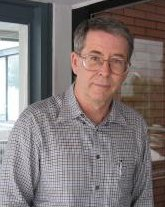
\includegraphics[height=30mm]{Aschbacher3}
\begin{center}
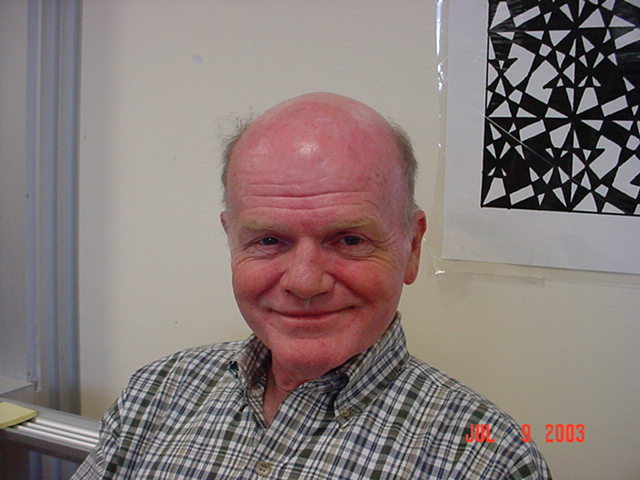
\includegraphics[height=25mm]{ONan}
\end{center}
\hfill    
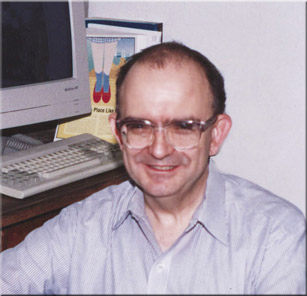
\includegraphics[height=28mm]{Scott}
%% %% \vskip3mm
%% \begin{center}
%% 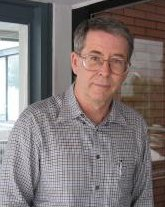
\includegraphics[height=29mm]{Aschbacher3}
%% \hskip2mm
%% 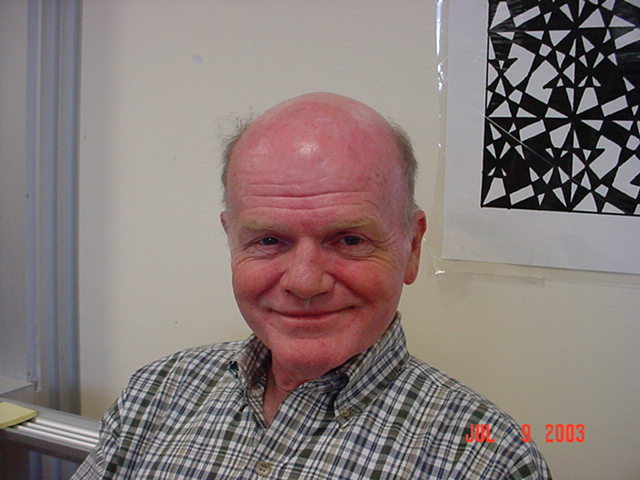
\includegraphics[height=25mm]{ONan}
%% \hskip2mm
%% %\hfill    
%% 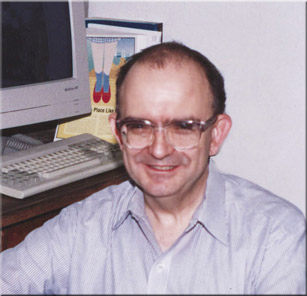
\includegraphics[height=28mm]{Scott}
%% \end{center}

\end{frame}

\begin{frame}[fragile,label=OSTheorem]{Aschbacher-O'Nan-Scott Theorem}
Let $G$ be a primitive permutation
group of degree $d$, and let $N := \Soc(G) \cong T^m$ with $m \geq 1$. 
Then one of the following holds.
\vskip2mm
\begin{enumerate}
\item 
$N$ is regular and
  \begin{itemize}
  \item 
  \alert{(Affine type)} $T$ is cyclic of order $p$, so $|N| = p^m$ . Then 
$d = p^m$ and $G$ is permutation isomorphic to a subgroup of the affine
general linear group $\AGL(m,p)$.
\vskip2mm
\item \alert{(Twisted wreath product type)} $m \geq 6$, the group $T$ is 
  nonabelian and $G$ is a group of \emph{twisted wreath product type}, with
  $d = |T|^m$.
  \end{itemize}
\vskip2mm
\item $N$ is non-regular, non-abelian, and
  \begin{itemize}
  \item 
\alert{(Almost simple type)} $m = 1$ and $T \leq G \leq \Aut(T)$.
\vskip2mm
\item \alert{(Product action type)} $m \geq 2$ and $G$ is permutation isomorphic to a
subgroup of the product action wreath product $P \wr S_{m/l}$ of degree
$d = nm/l$. The group $P$ is primitive of type 2.(a) or 2.(c), $P$ has
degree $n$ and $\Soc(P) \cong T^l$, where $l \geq 1$ divides $m$.
\vskip2mm
\item 
\alert{(Diagonal type)} $m \geq 2$ and $T^m \leq G \leq T^m . (\Out(T ) \times S_m)$, with
the diagonal action. The degree $d = |T|^{m-1}$.
  \end{itemize}
\end{enumerate}
\end{frame}

\begin{frame}[fragile,label=OSTheorem]{Aschbacher-O'Nan-Scott Theorem}
See Peter Cameron's blog at 
\begin{center}
{\small  \url{http://cameroncounts.wordpress.com/tag/onan-scott-theorem/}}
\end{center}
 for some history.
\end{frame}

\begin{frame}[fragile,label=FinalConclusions]{}
  \begin{center}
  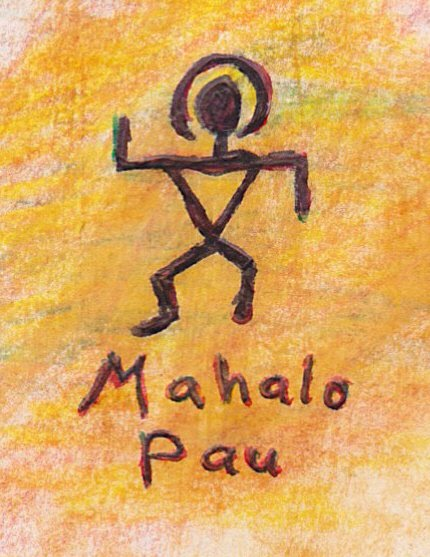
\includegraphics[height=2in]{MahaloPau}
  \end{center}
\end{frame}

















\begin{frame}[label=IEPropsLemma2Alt]{}
%\ifthenelse{\boolean{prezi}}{\FontLarge}{}
\alert{Proof Sketch}
\vskip2mm
  Let $L$ be a group representable lattice such that if $L\cong [H,G]$ and
  $\core_G(H)=1$ then $G$ is a $\cP$-group.  
\vskip4mm
  Since $L$ is representable, $\exists$ a $\cP$-group $G$ with $L
  \cong [H,G]$. 
\vskip4mm
\visible<2->{  We apply the idea of Hans Kurzweil twice.
  \begin{center}
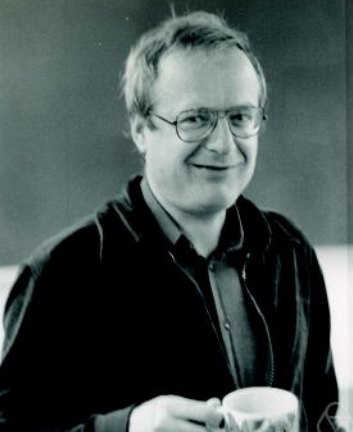
\includegraphics[height=3cm]{Kurzweil-crop}
  \end{center}
}
\end{frame}


\begin{frame}[label=IEPropsAlt2]{}
%\ifthenelse{\boolean{prezi}}{\FontLarge}{}
The following are at least cf-\IE: 
\vskip5mm
\begin{itemize}
\item $\sG_0 = \mathfrak{S}^c = $ the insoluble groups
\vskip2mm
\item $\sG_1 =\{G\in \G \mid (\forall n<\omega) \; (G \neq A_n \text{ and }  G\neq S_n) \}$
\vskip2mm
\item $\sG_2 = $ the subdirectly irreducible groups
\vskip2mm
\item $\sG_3 = $ groups with no nontrivial abelian normal subgroups
\vskip2mm
\item $\sG_4 = \{G\in \G \mid C_G(M) = 1 \text{ for all } 1\neq M\subnormal G\}$.
\end{itemize}
\vskip5mm
For $i= 2, 3, 4$,
\[\bH(\sG_i^c) \neq \sG_i^c\]
\end{frame}

\begin{frame}[label=IEPropsPrezi]{}
%\ifthenelse{\boolean{prezi}}{\FontLarge}{}
The following are at least cf-\IE: 
\vskip5mm
\begin{itemize}
\item $\sG_0 = \mathfrak{S}^c = $ the insoluble groups
\vskip2mm
\item $\sG_1 =\{G\in \G \mid (\forall n<\omega) \; (G \neq A_n \text{ and }  G\neq S_n) \}$
\vskip2mm
\item $\sG_2 = $ the subdirectly irreducible groups
\vskip2mm
\item $\sG_3 = $ groups with no nontrivial abelian normal subgroups
\vskip2mm
\item $\sG_4 = \{G\in \G \mid C_G(M) = 1 \text{ for all } 1\neq M\subnormal G\}$.
\end{itemize}
\end{frame}
\begin{frame}[label=IEPropsPreziAlt2]{}
%\ifthenelse{\boolean{prezi}}{\FontHuge}{}
\begin{center}
\vskip-4cm
Note that $\;\sG_4 \subset \sG_2\cap \sG_3 \subset \sG_0$.
\end{center}
\end{frame}

\begin{frame}[label=IEPropsPrezi]{}
%\ifthenelse{\boolean{prezi}}{\FontLarge}{}
\begin{center}
Note that $\;\sG_4 \subset \sG_2\cap \sG_3 \subset \sG_0$.
\end{center}
\vskip3cm
\begin{center}
$\bH(\sG_i^c) \neq \sG_i^c \quad \text{ for } \quad i= 2, 3, 4$
\end{center}
\end{frame}

\begin{frame}[label=IEPropsPrezi]{}
%\ifthenelse{\boolean{prezi}}{\FontLarge}{}
\begin{proof}
If $H\in \sG_i$ and $K\in \sG_i^c$ then,
$H\times K$ belongs to $\sG_i^c$, but
$(H\times K)/(1\times K) \cong H$ does not.
\end{proof}
\end{frame}

\begin{frame}[label=IEPropsPrezi]{}
%\ifthenelse{\boolean{prezi}}{\FontHuge}{}

\alert{Proof:}
\vskip4mm
 If $H\in \sG_i$ and $K\in \sG_i^c$ then,
\vskip4mm
$H\times K$ belongs to $\sG_i^c$, but
\vskip4mm
$(H\times K)/(1\times K) \cong H$ does not.

\end{frame}

\begin{frame}[label=IEPropsPrezi]{}
%\ifthenelse{\boolean{prezi}}{\FontHuge}{}

\alert{Proof:}
If $H\in \sG_i$ and $K\in \sG_i^c$ then,
$H\times K$ belongs to $\sG_i^c$, but
$(H\times K)/(1\times K) \cong H$ does not.
\end{frame}


\begin{frame}[label=IEPropsLemmaExtra]{}
%\ifthenelse{\boolean{prezi}}{\FontLarge}{}
\begin{lemma}
\label{lemma-wjd-2}
Suppose $\cP$ is a core-free interval enforceable property.  
If 
\[
\bH(\sG_{\cP}^c) = \sG_{\cP}^c
\]
then $\cP$ is an interval enforceable property.
\end{lemma}
\end{frame}

\begin{frame}[fragile,label=ASClass]{}
      \begin{center}
    {\scalefont{1.5}
        \begin{tikzpicture}[scale=.7]
                \node (bot) at (0,0)  [draw, circle, inner sep=1pt] {};
      \node (top) at (0,11)  [draw, circle, inner sep=1pt] {};
      \foreach \j in {-5,-3,-1,1,3,5} { 
        \node (\j4) at (\j,4)  [draw, circle, inner sep=1pt] {};
        \node (\j7) at (\j,7)  [draw, circle, inner sep=1pt] {};
        \draw[semithick] (bot) to (\j4)  (top) to (\j7);
      }
      \draw[semithick] (-54) to (-57) to (-34) to (-17) to (-14) to (-37) to (-54);
      \draw[semithick] (54) to (57) to (34) to (17) to (14) to (37) to (54);

        \end{tikzpicture}
}
      \end{center}
\end{frame}


\end{frame}

\begin{frame}[fragile,label=ExamplesPreziAschbacher]{}
  \begin{center}
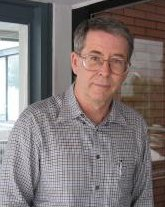
\includegraphics[height=6cm]{Aschbacher3}
  \end{center}
\end{frame}

\begin{frame}[fragile,label=ExamplesPreziShareshian]{}
  \begin{center}
\includegraphics[height=6cm]{Shareshian-clip}
  \end{center}
\end{frame}






\begin{frame}[label=P5Prezi]{}
%\ifthenelse{\boolean{prezi}}{\FontLarge}{}
      \begin{theorem}[{\small P\'alfy and Pudl\'ak, 1980}]
        The following statements are equivalent:
        \begin{itemize}
        \item[(i)] Every finite lattice is isomorphic to
          the congruence lattice of a finite algebra.
        \item[(ii)] Every finite lattice is isomorphic to
          an interval in the subgroup lattice of a finite group.
        \end{itemize}
      \end{theorem}
\end{frame}


\begin{frame}[fragile,label=OSTheorem]{Aschbacher-O'Nan-Scott Theorem}
%\ifthenelse{\boolean{prezi}}{\FontLarge}{}
See Peter Cameron's blog at 
\vskip5mm
\begin{changemargin}{+0cm}{-5mm}
{\small  \url{http://cameroncounts.wordpress.com/tag/onan-scott-theorem/}}
\end{changemargin}
\vskip5mm
 for some history.
\end{frame}














Michio Suzuki~\cite{Suzuki:1951} proved similar lattice theoretical
characterizations for soluble and perfect groups. 
More recently, 
John Shareshian and Russ Woodroofe~\cite{Shareshian:2012} prove that by comparing the lengths of certain maximal
chains in $\Sub(G)$ one can determine whether or not $G$ is soluble.



%% A lattice L is called sectionally complemented if for every b < c ∈ L there exists
%% a d ∈ L such that b ∧ d = 0 (the smallest element of the lattice) and b ∨ d = c. This
%% lattice theoretic property also has a neat group theoretic counterpart.
%% Theorem 2.9 (Bechtell [6], 1965) For a finite group G, the subgroup lattice Sub(G)
%% is sectionally complemented if and only if every Sylow subgroup of G is elementary
%% abelian.














%%%% Proof that subgroup at bottom of interval in Kurzweil construction is core-free %%%


  To complete the proof, we check that starting with a core-free subgroup
  $H \leq G$ in the Kurzweil construction just described results in a
  core-free subgroup $D \bar{G} \leq U$.   Let $N = \core_U(D\bar{G})$.  Then, for all $w=(d,\dots, d, x) \in N$ and for all 
  $u = (t_1,\dots, t_n, g)\in U$, we have $u w u^{-1}\in N$. 
  Fix $w=(d,\dots, d, x) \in N$.  We will choose $u\in U$ so that
  the condition $u w u^{-1}\in N$ implies $x$ acts trivially on $\{1, \dots, n\}$.
  First note that if $u = (t_1,\dots, t_n, 1)$, then
  %ll other $t_k$ distinct, and $g=1$.  
  \[
  u n u^{-1} = (t_1,\dots, t_n, 1) (d, \dots, d, x) (t_1^{-1},\dots, t_n^{-1}, 1)
  =(t_1 d \,t_{x(1)}^{-1},\dots, t_nd \,t_{x(n)}^{-1}, 1) \in N,
  \]
  and this implies that $t_1 d\, t_{x(1)}^{-1} = t_2 d\, t_{x(2)}^{-1} =\cdots = t_nd \,t_{x(n)}^{-1}$. 
  Suppose by way of contradiction that $x(1) = j\neq 1$.  Then, since $x$ is a
  permutation (hence, one-to-one), $x(k) \neq j$ for
  each $k\in \{2, 3, \dots, n\}$.  Pick one such $k$ other than $j$.
  (This is possible since $n = |G:H|>2$; for otherwise $H\subnormal G$
  contradicting $\core_G(H)=1$.) 
  Since $u \in U$ is arbitrary, we may assume
  $t_1 = t_k$ and $t_{x(1)}=t_j\neq t_{x(k)}$.  
  But this contradicts $t_1 d\, t_{x(1)}^{-1} = t_k d\, t_{x(k)}^{-1}$.
  Therefore, $x(1) = 1$.  The same argument shows that 
  $x(i) = i$ for each $1\leq i\leq n$, 
  and we see that
  $w=(d,\dots,d, x) \in N$ implies $x\in \ker \phi = 1$.  This puts $N$ below
  $D$, and the only normal subgroup of $U$ that lies 
  below $D$ is the trivial group.
\end{proof}









